\documentclass[12pt,UTF8]{ctexbook}
\usepackage{ctex}
\usepackage{caption}
\usepackage{graphicx}
\usepackage{float}
\usepackage{wrapfig}
\usepackage{array}
\usepackage[table, dvipsnames, svgnames, x11names]{xcolor}
\usepackage{colortbl}% 
\usepackage{tabularx}
\usepackage{amsmath, tikz}
\usepackage{amssymb}
\usepackage{xfrac}
\usepackage{eucal}
\usepackage{titlesec}
\usepackage{amsthm}
\usepackage{ifthen}
\usepackage{tikz-cd}
\usepackage{enumitem}
\usepackage{verbatim}
\usepackage{fontspec,xunicode,xltxtra}
\usepackage{pifont}
\usepackage{xeCJK} 

\definecolor{gl}{RGB}{246, 252, 240}
\definecolor{gd}{RGB}{236, 244, 230}
\definecolor{bg}{RGB}{242, 244, 228}


\setCJKmainfont[BoldFont=STZhongsong]{STSong}
\setCJKmonofont{simkai.ttf} % for \texttt
\setCJKsansfont{simfang.ttf} % for \textsf
\setlength\parskip{8pt}
\setlength{\fboxsep}{12pt}
\renewcommand\thesection{\arabic{chapter}.\arabic{section}}

\usetikzlibrary{calc,topaths}

\newcommand\widearc[1]{%
    \tikz[baseline=(wideArcAnchor.base)]{
        \node[inner sep=0] (wideArcAnchor) {$#1$}; 
        \coordinate (wideArcAnchorA) at ($(wideArcAnchor.north west) + (0.15em,0.1em)$);
        \coordinate (wideArcAnchorB) at ($(wideArcAnchor.north east) + (0.0em,0.1em)$);
    %
        \draw[line width=0.1ex,line cap=round,out=45,in=135] (wideArcAnchorA) to (wideArcAnchorB);
    }
}

% \newcommand{\jch}[2][]{
%     \begin{tikzpicture}[baseline]
%         \draw (-0.16em,0.32em) -- (0em,0.32em) -- (0em,-0.2em) -- (1em,-0.2em);  
%         \ifthenelse{\equal{$#1$}{}}{\node at (0.5em,0.3em) {$#1$}}{\node at (0.5em,0.3em) {$#2$}};
%         \ifthenelse{\equal{$#1$}{}}{}{\node at (0em,0.56em) {$\scriptscriptstyle #1$}};
%     \end{tikzpicture}
% }
\newtheorem{df}{定义}[section] 
\newtheorem{pp}{命题}[section]
\newtheorem{tm}{定理}[section]
\newtheorem{ex}{例子}[section]
\newtheorem{sk}{思考}[section]
\newtheorem{po}{公理}
\newtheorem*{ex*}{例子}
\newtheorem*{so}{解答}
\newtheorem*{proof2}{证明}
\newtheorem{xt}{习题}[section]
\newtheorem{cor}{推论}[pp]
\renewcommand{\proofname}{\indent\bf 证明}
\renewcommand{\qedsymbol}{\hfill$\square$}
% 列举环境的行间距
\setenumerate[1]{itemsep=0pt,partopsep=0pt,parsep=0pt,topsep=0pt}
\setitemize[1]{itemsep=0pt,partopsep=0pt,parsep=0pt,topsep=0pt}
\setdescription{itemsep=0pt,partopsep=0pt,parsep=0pt,topsep=0pt}
\setlength{\intextsep}{2pt}%
\setlength{\columnsep}{2pt}%
% 新函数
\renewcommand\parallel{\mathrel{/\mskip-4mu/}}
% 章节字体大小
\titleformat{\section}{\zihao{-2}\bfseries}{ \thesection }{16pt}{}
% 封面
\title{\zihao{0} \bfseries 第五册}
\author{\zihao{2} \texttt{大青花鱼}}
% \date{\bfseries\today}
\date{}
% 正文
\begin{document}
\maketitle
\tableofcontents
\newpage

\chapter{圆}

学习反比例函数和二次函数时,我们发现,就算是简单代数式定义的函数,它的图像也是我们无法手动画出的曲线。
曲线是比直线更复杂的形状。为了给我们今后研究各种曲线打下基础,以下我们研究一种简单的曲线:圆。

\section{圆的基本性质}
我们已经学过圆的概念。公理体系中,我们这样定义圆:平面上到定点$O$距离为定长的点的集合,是一个圆。
给定线段$XY$,到$O$的距离和$AB$等长的点构成一个圆。$O$叫做\textbf{圆心},
$XY$叫做圆的\textbf{半径},长度一般记为$r$。不至于混淆的时候,半径的长也简称为半径。

圆心为$O$、半径为$r$的圆,一般记为圆$(O, r)$或$\odot_{(O, r)}$。
圆心$O$和另一点$P$确定的圆,一般记为圆$(O, P)$或$\odot_{(O, P)}$。如果不在意半径,在不至于混淆的情况下,
也可以简记为圆$O$。

平面上的点到$O$的距离小于$r$,就说它在圆内;如果等于$r$,就说它在圆上;如果大于$r$,就说它在圆外。

和引进直线等概念时一样,圆也有一条公理,规定它和直线的关系。
\begin{po}\textbf{直线交圆公理}\label{po:0}
    直线和圆有两个交点,当且仅当直线有部分在圆内。
\end{po}

从这个公理出发,我们可以整理直线和圆的位置关系。

考虑直线$l$和圆$\odot_{(O, r)}$。过$O$作直线$m\perp l$,记垂足为$P$,$|OP| = d$。

\begin{figure}[h] %this figure will be at the right
    \vspace{8pt}
    \centering
    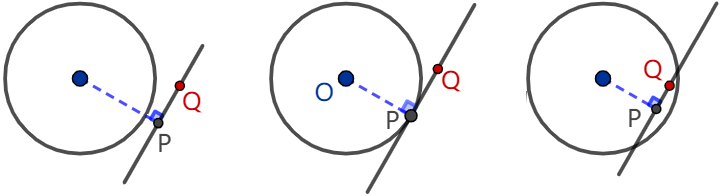
\includegraphics[width=0.72\textwidth]{圆与直线1.png}
\end{figure}

\begin{enumerate}
    \item 如果$d > r$,那么$P$在圆外。根据垂距定理,$l$上任意点都在圆外。我们说直线$l$与圆$O$\textbf{相离}。反之,如果直线与圆相离,那么$P$在圆外,因此$d > r$。
    \item 如果$d = r$,那么$P$在圆上。根据垂距定理,$l$上的点除了$P$都在圆外。直线和圆恰有一个公共点。我们说直线$l$与圆$O$\textbf{相切},称$P$为\textbf{切点}。
    反之,如果直线与圆相切于点$Q$,那么$|OQ| = r$。$l$上其他点都在在圆外,所以根据垂距定理的逆定理,$OQ \perp l$,$d = r$。
    \item 如果$d < r$,那么$P$在圆内。根据直线交圆公理,直线和圆有两个交点$A$、$B$。我们说直线与圆\textbf{相交},或直线\textbf{割圆}于$A$、$B$。
    反之,如果直线和圆有两个交点,那么根据直线交圆公理,直线有部分在圆内,这部分上的点到圆心距离小于$r$,因此根据垂距定理,$d < r$。
\end{enumerate}

设直线割圆于两点$A$、$B$,我们说直线是圆的\textbf{割线}。根据直线交圆公理,线段$AB$(除端点)在圆内。
我们把线段$AB$称为圆的一条\textbf{弦}。如果$AB$过圆心$O$,就说它是圆的直径,$A$、$B$互为\textbf{对径点}。
直径是过圆心的弦。它的长度是半径的两倍。不至于混淆的时候,直径的长也简称为直径。

考虑圆$O$上的弦$AB$的垂直平分线$m$,圆心$O$显然在$m$上。$m \perp AB$,设垂足为$P$,那么$|AP| = |PB|$。
设$m$和圆交于两点$C,D$,则弦$CD$就是直径。所以我们说:\textbf{恰有一条直径平分每条弦}。


% 考虑两个圆:$\odot_{(O_1, r_1)}$和$\odot_{(O_2, r_2)}$,设两个圆心的距离是:$|O_1O_2| = s$,
% 那么,两个圆的关系可能有以下几种:

% \begin{figure}[h] %this figure will be at the right
%     \vspace{8pt}
%     \centering
%     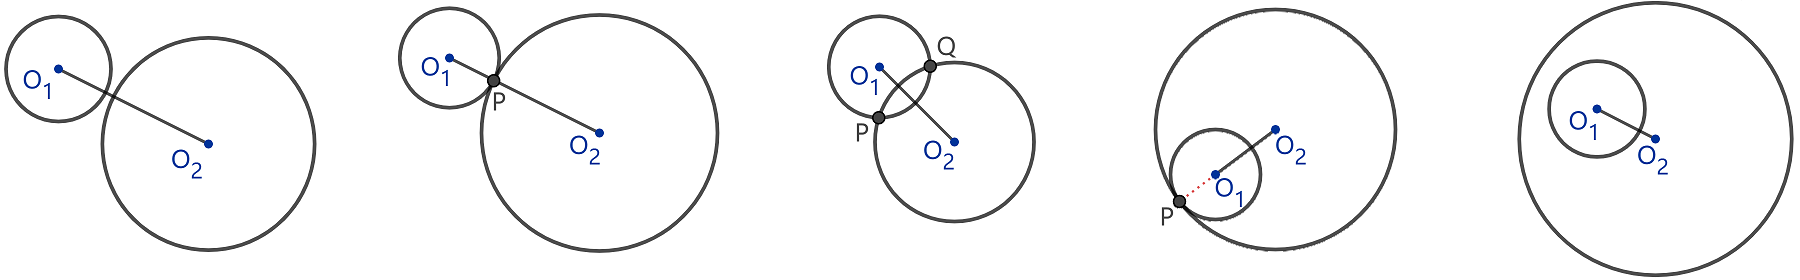
\includegraphics[width=0.9\textwidth]{圆与圆1.png}
% \end{figure}

% \begin{enumerate}
%     \item $s > r_1 + r_2.$ 用反证法可以证明,两个圆没有公共点。我们说两圆\textbf{相离}。
%     \item $s = r_1 + r_2.$ 考虑线段$O_1O_2$,上面有一点$P$使得$|O_1P| = r_1$,于是$|PO_2| = |O_1O_2| - |O_1P| = r_2$。
%     这说明两个圆有一个公共点。如果点$Q$不在线段$O_1O_2$上,则$|O_1Q| + |QO_2| > |O_1O_2|$。
%     于是$Q$不可能是公共点。也就是说,两个圆恰有一个共同点,在圆心连线上。我们说两圆\textbf{外切}。
%     \item $|r_1 - r_2| < s < r_1 + r_2.$ 根据第二个公理,$\odot_{(O_1, r_1)}$和$\odot_{(O_2, r_2)}$恰有两个公共点,分别在圆心连线两侧。我们说两圆\textbf{相交}。
%     \item $s = |r_1 - r_2|.$ $r_1 > r_2$时,$s = r_1 - r_2$。考虑直线$O_1O_2$,上面有一点$P$,使得$|O_1P| = r_1$,且和$O_2$在$O_1$同一边。于是$|O_2P| = |O_1P| - |O_1O_2| = r_2$。
%     这说明两个圆有一个公共点。如果点$Q$不在线段$O_1O_2$上,则$|O_1O_2| + |QO_2| < |O_1Q|$。
%     于是$Q$不可能是公共点。也就是说,两个圆恰有一个共同点,在圆心连线上。$r_1 > r_2$时,通过类似推理可以得到同样的结论。我们说两圆\textbf{内切}。
%     \item $s < |r_1 - r_2|.$ 用反证法可以证明,两个圆没有公共点。如果$r_1 > r_2$,我们说$\odot_{(O_1, r_1)}$\textbf{内含}$\odot_{(O_2, r_2)}$,$\odot_{(O_2, r_2)}$\textbf{内含于}$\odot_{(O_1, r_1)}$;反之亦然。
% \end{enumerate}
% 要注意的是,如果仅知道两圆恰有一个公共点,我们无法判断到底是第二还是第四种情形;如果仅知道两圆没有公共点,我们无法判断到底是第一还是第五种情形。
% 第二和第四种情形可以统称为两圆\textbf{相切},第一和第五种情形可以统称为两圆\textbf{相离}。
    % \indent 2. 完成两圆关系的第一和第五种情形中的证明。\\
    % \indent 3. 阐明两圆关系的第四种情形中,$r_1 > r_2$情况下的推理过程。

\begin{xt}\label{xt:0-0-0}
    补充:\\
    \indent 1. 设直线割圆于两点$A$、$B$,证明线段$AB$(除端点)在圆内。\\
    \indent 2. 证明:同一个圆中,直径是最长的弦。
\end{xt}

\section{圆和旋转}
怎么画一个圆?我们用圆规画圆。如果已知圆心和圆上一点,我们将圆规尖定在要画的圆心处,
将笔头接触圆上的点,然后轻轻旋转,笔头就画出一个圆。如果已知圆心和半径线段,我们首先张开圆规,
圆规尖和笔头分别对齐半径两端,然后保持圆规形状不变,将圆规尖定在要画的圆心处,让笔头接触纸面,
轻轻旋转,笔头就画出一个圆。

可以看出,圆和旋转有天然的关系。旋转是由角定义的操作,把平面中的点映射到另一点。
给定角$AOB$,可以这样定义\textbf{旋转}:

\begin{df}\label{df:0-1-0}
    给定角$AOB$,平面中一点$P$关于$\angle AOB$旋转的结果,
    是唯一使得$\angle POQ = \angle AOB$且$|OP| = |OQ|$的点$Q$。
\end{df}
$O$称为旋转的\textbf{中心}。任何点$P$绕中心旋转,结果都在圆$(O,P)$上。

可以看到,给定一个圆$(O,P)$,从点$P$出发,旋转不同的角度,
就得到圆上其它的点。用圆规画圆时,从零角出发,随着角度不断增大,直到周角,我们沿逆时针经历了圆上所有的点
(注意:这里约定角度的范围是$0^\circ$到$369^\circ$)。
也就是说,我们认为零角到周角的角按角度和圆上的点之间有一一映射。
换句话说,数轴上$0$和$360$之间的数,和圆上的点之间有一一映射。
我们把它称作\textbf{圆映射},记为$\gamma_{(O,P)}$。

通过$\gamma_{(O,P)}$,我们可以把对圆的研究,改为对数轴上线段的研究。
这样就把曲线上的问题转为了直线上的问题。
比如,既然$[0, 360)$对应整个圆,那么$[0,180]$就对应半个圆,
$[0,60]$就对应六分之一个圆,等等。我们把闭区间对应的圆的部分称为\textbf{圆弧}。

同一圆上两个圆弧分别对应$[\, a_1, a_1+x\, ]$和$[\, a_2, a_2+x \,]$,这两个圆弧有什么不同吗?
观察圆的图像可知,并没有不同。也就是说,圆弧的形状只和它对应数轴上区间的长度有关,和它所在的位置无关。
只要对应的区间一样长,那么圆弧就全等,可以相互覆盖。换句话说,圆弧只要等长,就是全等的。
于是,线段所满足的公理,对同一个圆上的圆弧也成立。

和线段一样,圆弧也有起点和终点。比如$[\, 0,60\, ]$对应的圆弧,起点就是$P$,
终点是$60$度角$POQ$的终边和圆的交点$Q$。如果圆弧对应的区间长度超过$180$,就说它是\textbf{优弧};
如果圆弧对应的区间长度小于$180$,就说它是\textbf{劣弧};如果等于$180$,就说它是\textbf{半圆}。
优弧比半圆长,劣弧比半圆短。

从直线和圆相交的角度来看,圆上两点确定的直线将圆分为两个圆弧。这两个圆弧并起来就是圆,
所以要么一个是优弧、一个是劣弧,要么两者都是半圆(这时直线过圆心)。我们说它们互为\textbf{补弧}。

同一个圆上,明确了起点$A$和终点$B$,就唯一确定了圆弧$\widearc{AB}$。如果只说了两点$A$、$B$,
那么$\widearc{AB}$一般指劣弧或起点为$A$终点为$B$的圆弧。

\begin{xt}\label{xt:0-1-0}
    证明:\\
    \indent 1. 任意线段经过旋转得到等长的线段。\\
    \indent 2. 任意三角形经过旋转得到同角全等的三角形。 
\end{xt}

\section{圆心角和圆周角}

根据圆映射的定义,每个圆弧都对应一个顶点在圆心,大小介于零角和周角之间的角,称为它的\textbf{圆心角}。
圆弧还可以对应另一类角。给定起点为$A$,终点为$B$的圆弧$\widearc{AB}$和圆上弧外一点$P$,
则角$APB$称为一个\textbf{圆周角}。
每个圆弧只对应一个圆心角,但可以对应很多个圆周角。

同一段圆弧的圆心角和圆周角之间,有什么关系呢?如右图,连接$PO$,延长交圆于对径点$Q$。
由于$\triangle AOP$是等腰三角形,$\angle OAP + \angle OPA = 0$,
同理,$\angle OBP + \angle OPB = 0$。于是
\begin{align}
    \angle AOB &= \angle AOQ + \angle QOB \notag \\ 
    &= \angle OAP + \angle APO + \angle PBO + \angle OPB \notag \\
    &= 2\angle APO + 2\angle OPB = 2\angle APB \notag
\end{align}
也就是说,圆心角是圆周角的两倍大小,圆周角是圆心角的一半大小。

\begin{tm}\textbf{圆周角定理}\label{tm:0-2-0}
    给定圆$O$上的弧$\widearc{AB}$及圆上弧外的点$P$,如果$P \notin \widearc{AB}$,那么:
    $$\angle APB = \frac{1}{2} \angle AOB,$$
\end{tm}

如果点$P$在弧上,$\angle APB$和$\angle AOB$是什么关系呢?
这时$\angle APB$对应$\widearc{AB}$的补弧,于是它
是$\widearc{AB}$对应的圆心角的一半大小。$\widearc{AB}$对应的圆心角是周角减去$\angle AOB$,所以
$$\angle APB = 180^\circ - \frac{1}{2} \angle AOB.$$

对径点和圆心形成平角,因此,根据圆周角定理,对径点对应的圆周角是直角。或者说,半圆对应的圆周角是直角。

要注意的是,讨论圆心角时,我们约定角的范围是零角到周角。讨论圆周角和其他角时,为了方便,我们会切换到
负平角到正平角的范围。

同一个圆里,圆上的点$A$、$B$对应的圆心角$\angle AOB$和点$C$、$D$对应的圆心角$\angle COD$相等,那么
根据“边角边”,圆心$O$和它们构成的三角形满足:$\triangle AOB \simeq \triangle COD$。弦$AB$和$CD$也等长。
不仅如此,根据圆映射,圆弧$\widearc{AB}$和$\widearc{CD}$也等长。
事实上,$\widearc{CD}$就是$\widearc{AB}$关于某个角旋转的结果。
我们把这个结论称为“等角对等弦”、“等角对等弧”。

反之,如果两个圆弧$\widearc{AB}$和$\widearc{CD}$等长,那么它们对应的区间也一样长。
这说明它们对应的圆心角一样大。
圆心角既然相等,那么弦$AB$和$CD$也等长。
更进一步,设$P$是圆上不属于两弧的点,那么圆周角$\angle APB$和$\angle CPD$一样大。我们把这个结论称为“等弧对等弦”、“等弧对等角”。

反过来,如果圆$O$上两条弦$AB$和$CD$等长,那么根据“边边边”,$\triangle AOB \simeq \triangle COD$。
于是圆心角相等,所以劣弧$\widearc{AB}$和$\widearc{CD}$等长。我们把这个结论称为“等弦对等角”、“等弦对等弧”。

总的来说,在同一个圆里,两点对应的弦长相等当且仅当对应的(劣弧)弧长相等,当且仅当对应的圆心角相等,
当且仅当对应的圆周角相等。弦、弧、圆心角、圆周角,都是用来描述圆的部分和整体关系的方法。

给定圆上两点$A$、$B$,它们对应的垂直平分线$l$平分$\angle AOB$,即把$\angle AOB$分成两个相同大小的圆心角。
因此,设$l$和圆交于$P$、$Q$,则它们也分别平分所在的圆弧(称为弧的中点)。
我们把这一系列结论总称为垂径定理:
\begin{tm}\textbf{垂径定理 }\label{tm:0-2-1}
    给定圆上两点,则恰有圆的一条直径垂直平分两点对应的弦,同时平分对应的圆心角和两个圆弧。
\end{tm}
垂径定理也可以说成:过圆$O$的弦$AB$中点的直径与弦$AB$垂直,同时平分$\angle AOB$和弧$\widearc{AB}$。

给定圆$(O, r)$,弦$AB$中点记为$M$,$|MO|$称为弦$AB$的\textbf{弦心距}。由于$MO \perp AB$,
$\triangle OAM$是直角三角形,根据勾股定理,
$$|OM|^2 + |AM|^2 = |OA|^2 = r^2.$$
设直线$MO$与圆$O$交于$P$、$Q$两点,则
$$|MP| \cdot |MQ| = (r - |OM|)(r + |OM|) = r^2 - |OM|^2.$$
比较以上两式,可以得到:
$$ |MA| \cdot |MB| = |MA|^2 = |MB|^2 = |MP| \cdot |MQ|.$$
这个推论也常常被称为垂径定理。

\section{点到圆的势}
圆是到定点距离相同的点的集合,所以点对圆来说是关键的概念。
一点和圆的关系,可以用它到圆的距离来理解。点$P$在圆$(O, r)$上,当且仅当它到圆心的距离为$r$。

如果不知道圆心的位置,有没有办法理解点和圆的位置关系呢?
我们引进点到圆的\textbf{势}的概念。

\begin{df}
   点$P$到圆$(O, r)$的势,等于$|OP|^2 - r^2$。 
\end{df}

乍一看,点到圆的势,仍然和它到圆心的距离相关。点到圆心的距离$d$比$r$小的时候,点在圆内,
这时它到圆的势小于$0$。$d>r$的时候,点在圆外,势也大于$0$。$d=r$的时候,点在圆上,
势等于$0$。

下面,我们从垂径定理出发,给出一种不依赖圆心的方法,计算点到圆的势。

首先设点$P$在圆$(O,r)$内。连接$OP$,延长为直径,交圆于$A,B$两点($A$、$P$在$O$同侧)。
过$P$作该直径的垂线,交圆于$C,D$两点。弦$CD$的垂直平分线过$O$,而$OP \perp CD$,
所以$OP$就是弦$CD$的垂直平分线。根据垂径定理,$|PA|\cdot|PB| = |PC| \cdot |PD| = r^2 - |OP|^2$。
这说明$|PA|\cdot|PB|$、$|PC| \cdot |PD|$是$P$的势的绝对值。

过$P$任意作一条直线,和圆交于两点$M,N$,是否也有这个结论呢?

\begin{wrapfigure}[7]{r}{0.43\textwidth} %this figure will be at the right
    \vspace{-22pt}
    \flushright
    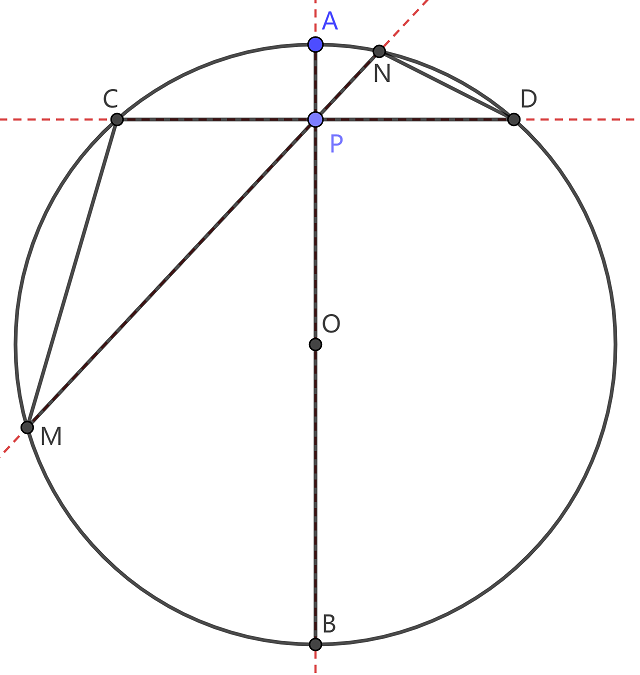
\includegraphics[width=0.42\textwidth]{圆势1.png}
\end{wrapfigure}

如右图,可以发现,$\angle NDC$和$\angle NMC$都对应同一段弧,且$C,M$都在弧外,
所以$\angle NDC = \angle NMC$。又对顶角$\angle DPN = \angle CPM$,所以
$ \triangle DPN \backsim \triangle MPC$。也就是说,
$$ \frac{|PD|}{|PN|} = \frac{|PM|}{|PC|}.$$
换句话说,$|PC| \cdot |PD| = |PN|\cdot|PM|$。这个结论也叫\textbf{相交弦定理}。

对圆内一点$P$来说,即便不知道圆心,只要过$P$作直线与圆交于两点,那么$P$到两点的距离乘积
就是它到圆的势的绝对值。

如果点在圆外,是否有类似的结论呢?我们仍然连接$OP$,直线$OP$割圆于两点:$A,B$
($A$位于$O$、$P$之间)。可以算出:
$$|PA|\cdot|PB| = (|PO| - |AO|) \cdot (|PO| + |PB|) = |OP|^2 - r^2.$$
过$P$作直线$l$和圆交于两点$M,N$,$|PM| \cdot |PN|$是否也等于$|OP|^2 - r^2$呢?

\begin{wrapfigure}[12]{r}{0.43\textwidth} %this figure will be at the right
    \vspace{-18pt}
    \flushright
    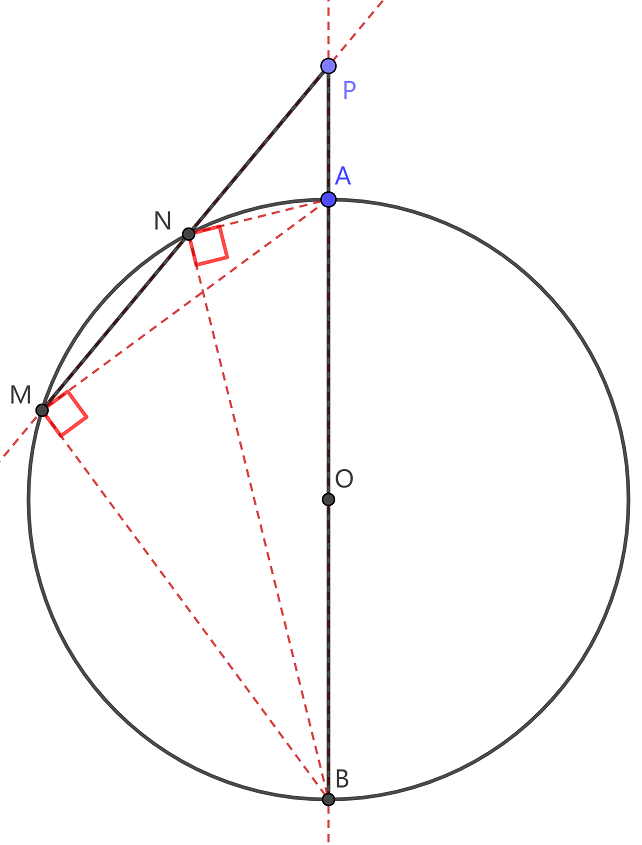
\includegraphics[width=0.42\textwidth]{圆势2.png}
\end{wrapfigure}

如右图,注意到$\angle BNA$和$\angle BMA$都对应半圆,所以都是直角。
三角形外角$\angle PAN = \angle ABN + \angle BNA$,而$\angle ABN$和$\angle AMN$对应同一段弧且都不在弧上,
所以$\angle ABN = \angle AMN$。于是,
\begin{align}
    \angle PAN &= \angle ABN + 90^\circ \notag \\
    &= \angle AMN + \angle BMA =\angle BMN. \notag
\end{align}
这说明$\triangle PAN \backsim \triangle PBM$,所以
$$ \frac{|PA|}{|PN|} = \frac{|PM|}{|PB|},$$
换句话说,$|PM|\cdot |PN| = |PA|\cdot |PB|$。
这个性质也叫\textbf{割线定理}。

对圆外一点$P$,即便不知道圆心,只要过$P$作直线与圆交于两点,那么$P$到两点的距离乘积
就是它到圆的势。

因此,无论在圆内还是圆外,经过一点$P$的直线与圆交于两点,则它到两点的距离乘积只与它和圆的远近关系有关。
如果$P$在圆内,这个乘积等于$r^2 - |PO|^2$;如果$P$在圆外,这个乘积等于$|PO|^2 - r^2$。
或者说,这个乘积就是势的绝对值。至于$P$在圆上的情形,我们可以认为它与圆交于两点,其中一点就是它自身,
所以到自身距离为$0$,从而乘积总是$0$,等于它的势。

\begin{tm}\textbf{圆势定理}\label{tm:0-3-40}
    过点$P$作直线与圆$(O, r)$交于两点:$A$、$B$,那么
    $$ |PA| \cdot |PB| = \left||PO|^2 - r^2\right|. $$
\end{tm}

比起乘积$|PA| \cdot |PB|$,点到圆的势多了正负号。如何理解这个正负号呢?如果过圆$(O,r)$的圆心
作一条直线,在上面建立数轴。当我们把原点$P$选在圆内的时候,$A$和$B$就对应符号相异的数;如果
把原点$P$设在圆外,$A$和$B$就代表同号的数了。
所以,以$P$为原点,$PO$为正方向的数轴和圆交于两点,这两点代表的数的乘积就是$P$到圆的势。
或者说,圆势附带了$P$和$A$、$B$的位置关系的信息。


\section{切线}
过一点作直线要与圆交于两点不难,与圆交于一点则不简单。
根据直线交圆公理,过圆内的点,无法作和圆相切的直线。过圆外一点,可以作与圆相切的直线
直观上,我们可以把直尺从和圆相交的状态逐渐移动,直到尺子碰到圆的“边缘”,作出大致和圆相切的直线。

直线和圆相切是一种特殊的状况。过圆外或圆上一点的直线$l$如果和圆$O$相切,就说它是点到圆的\textbf{切线}。
切线和圆的(唯一)交点,称为\textbf{切点}。根据相切的性质,过圆心$O$作关于$l$的垂线,切点就是垂足。
过圆上一点,只有一条切线,过圆外一点,可以作两条切线。

过圆$(O,r)$外一点$P$作切线,记切点为$Q$,则$\triangle OQP$为直角三角形。根据勾股定理,
$$ |PQ|^2 + |OQ|^2 = |OP|^2.$$
因此,$|PQ|^2 = |OP|^2 - r^2$。也就是说,点$P$到切点的距离平方,
是它关于圆的势。若过$P$作圆$O$的割线,交圆于$A$、$B$两点,那么
$$ |PA| \cdot |PB| = |OP|^2 - r^2 = |PQ|^2.$$
也就是说,
$$ \frac{|PA|}{|PQ|} = \frac{|PQ|}{|PB|}.$$
因此,$\triangle PAQ \sim \triangle PQB$。这两个三角形的相似关系称为\textbf{切割线定理}。
切割线定理可以看作割线定理的特例。

从切割线定理可以推出:$\angle PQA = \angle PBQ$。从另一个角度,可以这样理解:
过圆上一点$Q$只有一条切线$PQ$。如果过$Q$再作一条直线,直线于圆必交于另一点$A$,
而$\angle PQA$等于圆弧$\widearc{QA}$对应的圆周角。

\begin{sk}\label{sk:0-4-0}
    已知圆外一点$P$,如何准确作出$P$到$O$的切线?
\end{sk}


\chapter{圆和多边形}
我们对圆上一点、两点引出的形状都有了初步了解,现在来看圆上多个点对应的形状。

\section{三角形的外接圆和内切圆}
首先来看三个点的情形。

设$A$、$B$、$C$是圆$(O,r)$上(相异的)三点,则线段$AB$、$BC$、$AC$的垂直平分线都过圆心$O$。
因此,$O$是$\triangle ABC$的外心(这里附带说明了圆上相异三点必然不共线),$|OA|=|OB|=|OC|=r$。
反之,设有(非退化的)$\triangle ABC$,以它的外心$O$为圆心,以$|OA|$为半径,就可以画出一个圆,
过顶点$A$、$B$、$C$。这说明,\textbf{不共线的三点恰好对应一个圆}。或者说,\textbf{不共线的三点确定一个圆}。
我们把这个圆称为三角形的\textbf{外接圆}(“外心”即“外接圆圆心”的简称),把三角形称为圆的\textbf{内接三角形}。

三角形不仅可以内接于圆,圆也可以内接于三角形。考虑三角形$ABC$的内心,它到三角形三边的距离相等。
以内心为圆心,以它到三边的距离为半径作圆,这个圆和三角形三边都相切。我们把这个圆叫做三角形的\textbf{内切圆}
(“内心”即“内切圆圆心”的简称),把三角形称为圆的\textbf{外切三角形}。

\begin{wrapfigure}[7]{r}{0.46\textwidth} %this figure will be at the right
    \vspace{-20pt}
    \flushright
    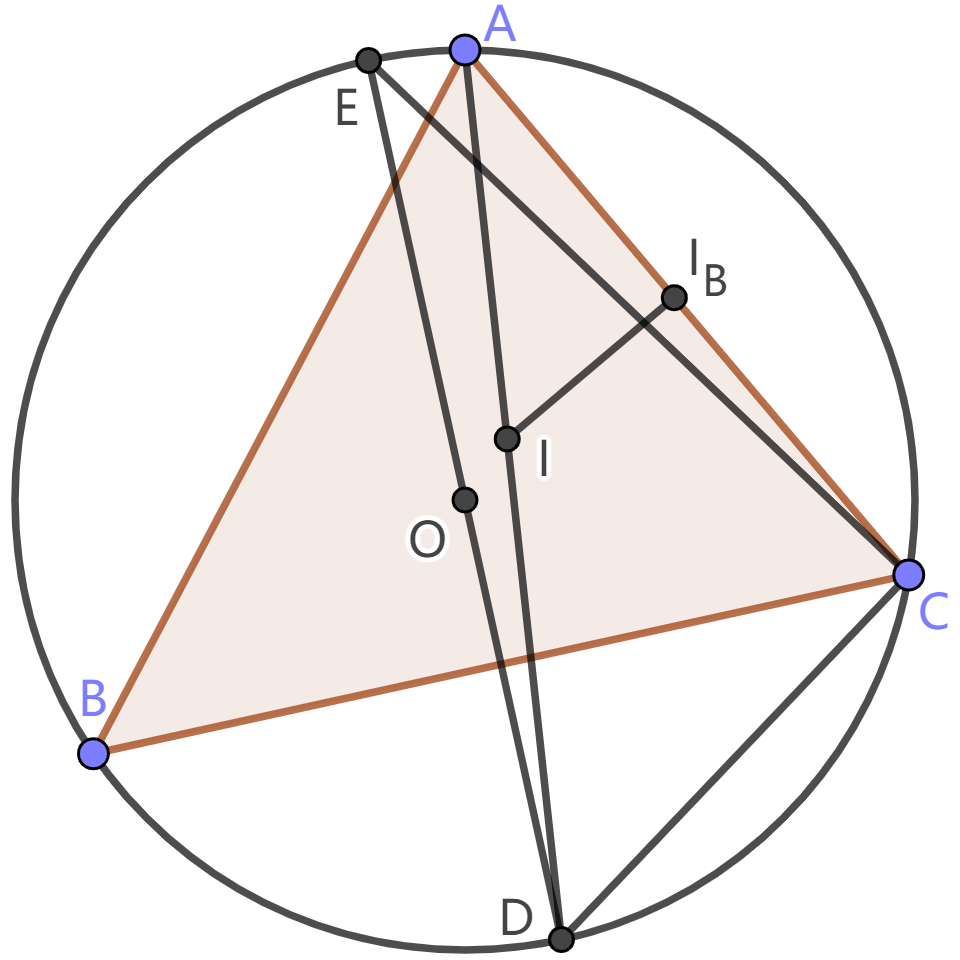
\includegraphics[width=0.45\textwidth]{内切圆势1.png}
\end{wrapfigure}

除了内心,三角形还有旁心。旁心到三角形三边的距离也相等。因此,以每个旁心为圆心,以它到三遍的距离为圆心,
各可以得到一个圆。每个圆都与三角形一边和另两边的延长线相切。这三个圆称为三角形的旁切圆
(“旁心”即“旁切圆圆心”的简称),把三角形称为它们的\textbf{旁切三角形}。

\begin{xt}\label{xt:1-0-10}
    \mbox{} \\
    如右上图,$\triangle ABC$的内心为$I$,外心为$O$。设$I$到$AC$的垂足为$I_B$,
    射线$AI$与圆$O$交于$D$,$D$的对径点为$E$。\\
    \indent 1. 证明:$\triangle CDI$是等腰三角形,$|CD| = |DI|$。\\
    \indent 2. 证明:$\triangle CDE \sim \triangle I_BIA$。\\
    \indent 3. 证明:$I$关于圆$O$的势$\mathtt{R}^2 - |OI|^2 = 2\mathtt{Rr}$。其中$\mathtt{R}$是外接圆半径,
    $\mathtt{r}$是内切圆半径。\\
    \indent 4. 设$J_A, J_B, J_C$是$\triangle ABC$的旁心,证明:它们关于圆$O$的势分别等于外接圆半径与对应旁切圆半径乘积的两倍。
\end{xt}

\section{圆内接四边形}
在三个点的基础上再加一个点$D$,四个点$A$、$B$、$C$、$D$能否恰好对应一个圆呢?显然,
$\triangle ABC$和$\triangle BCD$的外接圆未必是同一个圆。所以,四个点不总是在同一个圆上。
换句话说,要让四个点共圆,这四个点必须满足一定的条件。

\begin{wrapfigure}[3]{r}{0.32\textwidth} %this figure will be at the right
    \vspace{-40pt}
    \flushright
    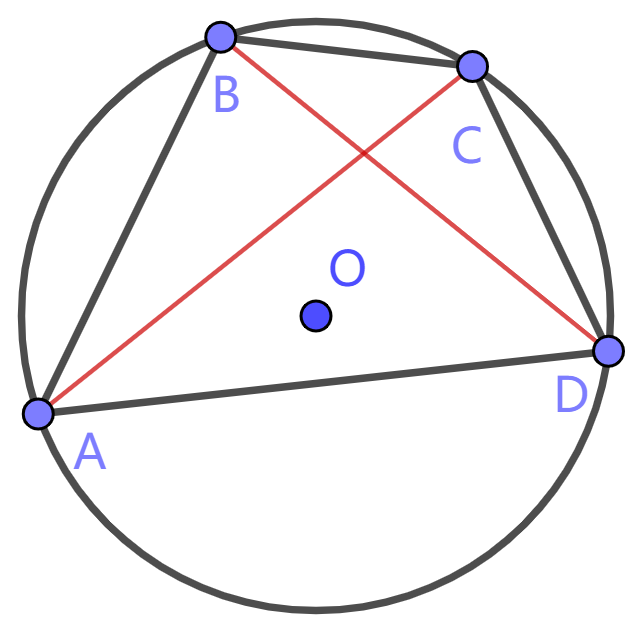
\includegraphics[width=0.3\textwidth]{圆内接四边形1.png}
\end{wrapfigure}

如右图,设$A$、$B$、$C$、$D$圆$(O,r)$上(相异的)四点,考察它们对应的圆弧。我们发现,
$\widearc{ABC}$和$\widearc{CDA}$是整个圆的分划,因此,它们对应的圆心角之和是周角。
根据圆周角定理,$\angle ABC + \angle CDA = 180^\circ$。同理,$\angle BCD + \angle DAB = 180^\circ$。

我们还可以发现,圆周角$\angle BAC$和$\angle BDC$都对应$\widearc{BC}$,因此根据“等弧对等角”,
$\angle BAC = \angle BDC$。同理可得:$\angle ACB = \angle ADB$,$\angle CAD = \angle CBD$,
$\angle DBA = \angle DCA$。

% 从这些等角关系出发,
% 如果对角线$AC$和$BD$交于点$P$,那么$\triangle APB \backsim \triangle CPD$、$\triangle BPC \backsim \triangle DPA$。

\begin{wrapfigure}[4]{r}{0.32\textwidth} %this figure will be at the right
    \vspace{-48pt}
    \flushright
    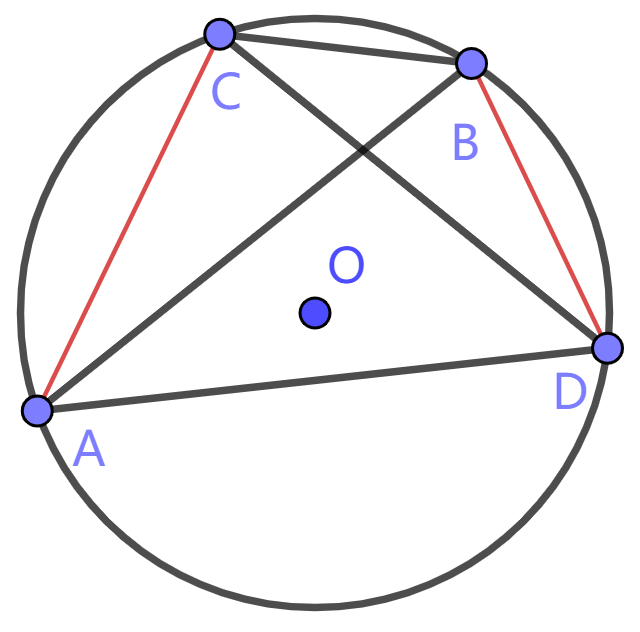
\includegraphics[width=0.3\textwidth]{圆内接四边形1b.png}
\end{wrapfigure}

如果$A$、$B$、$C$、$D$顺序改变,如右图,那么四边形$ABCD$就是蝶形。
$\widearc{ABC}$和$\widearc{CDA}$对应同一段圆弧$\widearc{AC}$。
这时$\angle ABC + \angle CDA = 0^\circ$,或者说$\angle ABC = \angle ADC$。
同理,$\angle BAD = \angle BCD$。

综合两种情况,\textbf{圆内接四边形对角要么和为平角,要么相等}。

可以看到,如果把相交的对边
$AB$、$CD$看作对角线,把对角线$AC$、$BD$看作对边,我们就得到一个凸四边形$ACBD$。
因此,观察相同的圆弧对应的圆周角可以发现,我们仍然有$\angle BAC = \angle BDC$、$\angle ACB = \angle ADB$,$\angle CAD = \angle CBD$,
$\angle DBA = \angle DCA$。如果对角线$AC$和$BD$交于点$P$,仍然有$\triangle APB \backsim \triangle CPD$、$\triangle BPC \backsim \triangle DPA$。
换句话说,即便圆内接四边形不是凸四边形,用它的顶点也能画出圆内接凸四边形,并且不妨碍我们讨论相关的性质。
所以,我们总把圆内接四边形问题归结为凸四边形来讨论,也称之为四点共圆问题。

以上是圆内接四边形边和角的性质,反过来,满足什么性质的四边形是圆内接四边形呢?
或者说,满足什么条件的四个点共圆呢?

\begin{tm}\label{tm:1-1-0}
    如果凸四边形$ABCD$中的一对内角$\angle ABC$与$\angle CDA$的和是平角,
    那么$ABCD$是圆内接四边形。
\end{tm}

\begin{proof}
    $\angle ABC + \angle CDA = 180^\circ$,所以要么两个角都是直角,要么一个是钝角,一个是锐角。\\
    如果两个角都是直角,作对角线$AC$,取它的中点$O$。$\triangle ABC$是直角三角形,$AC$是斜边,
    根据直角三角形的中线定理,$|AO| = |BO| = |CO|$。同理,$\triangle CDA$是直角三角形,$AC$是斜边,
    于是$|AO| = |DO| = |CO|$。因此$A,B,C,D$四点都在$\odot_{(O, A)}$上。\\
    如果两个角一个是钝角,一个是锐角。不妨设$\angle ABC > 90^\circ > \angle CDA$。作对角线$AC$,
    则$B$、$D$在$AC$两侧。作对角线$AC$的垂直平分线$l$。
    显然,$\triangle ABC$和$\triangle CDA$的外心都在$l$上,只需证明两者是同一点。\\
    设$\triangle ABC$的外接圆为$\odot_{(O_1, B)}$。$\angle ABC$是钝角,因此它的圆心角对应优弧。
    于是,$O_1$和$B$在直线$AC$两侧。$\angle CO_1A = 360^\circ - 2\angle ABC$。\\
    另一方面,设$\triangle CDA$的外接圆为$\odot_{(O_2, D)}$。$\angle CDA$是锐角,因此它的圆心角对应劣弧。
    于是,$O_2$和$D$在直线$AC$同一侧。$\angle CO_2A = 2\angle CDA$。\\
    以上两个结论说明,$O_1$和$O_2$都和$D$在直线$AC$同一侧,且$\angle CO_1A = \angle CO_2A$。
    而$\triangle CO_1A$和$\triangle CO_2A$都是等腰三角形,所以两者同角全等。这说明$O_1$和$O_2$是同一点。
    $A,B,C,D$四点都在$\odot_{O_1, A}$上。
\end{proof}

从这个定理可以推出,矩形、等腰梯形和正方形都是圆内接四边形。

\begin{tm}\label{tm:1-1-10}
    如果凸四边形$ABCD$中,$\angle ACB = \angle ADB$,
    那么$ABCD$是圆内接四边形。
\end{tm}

\begin{proof}
    $ABCD$是凸四边形,所以$C$和$D$在直线$AB$同侧。
    作边$AB$的垂直平分线$l$,显然,$\triangle ABC$和$\triangle ABD$的外心都在$l$上,
    只需证明它们是同一点。\\
    设$\triangle ABC$的外接圆为$\odot_{(O_1, C)}$,
    $\triangle ABD$的外接圆为$\odot_{(O_2, D)}$。
    如果$\angle ACB$是钝角,那么它的圆心角对应优弧。
    于是,$O_1$和$C$在直线$AB$两侧,且$\angle BO_1A = 360^\circ - 2\angle ACB$。
    这时,$\angle ADB = \angle ACB$也是钝角,所以同样有$O_2$和$D$在直线$AB$两侧,且
    $\angle BO_2A = 360^\circ - 2\angle ADB$。
    如果$\angle ACB$是锐角,那么它的圆心角对应劣弧。
    于是,$O_1$和$C$在直线$AB$同侧,且$\angle BO_1A = 2\angle ACB$。
    这时,$\angle ADB = \angle ACB$也是锐角,所以同样有$O_2$和$D$在直线$AB$同侧,且
    $\angle BO_2A = 2\angle ADB$。\\
    因此,$O_1$和$O_2$总在直线$AB$同侧,且$\angle BO_1A = \angle BO_2A$。
    而$\triangle BO_1A$和$\triangle BO_2A$都是等腰三角形,所以两者同角全等。这说明$O_1$和$O_2$是同一点。
    $A,B,C,D$四点都在$\odot_{O_1, A}$上。
\end{proof}

\begin{tm}\label{tm:1-1-20}
    过一点$P$的两条直线$m,n$上各有两点:$A, C\in m$和$B, D \in n$,分别各在$P$两侧。
    如果
    $$ |PA| \cdot |PC| = |PB| \cdot |PD|, $$
    那么四边形$ABCD$是圆内接四边形。
\end{tm}

\begin{proof}
    考虑$\triangle APB$和$\triangle DPC$。对顶角$\angle APB = \angle DPC$。
    而$ |PA| \cdot |PC| = |PB| \cdot |PD|$等于说
    $$ \frac{|PA|}{|PB|} = \frac{|PD|}{|PC|}.$$
    因此根据“边角边”,$\triangle APB \sim \triangle DPC$。于是有
    $\angle ABP = \angle DCP$,$\angle BAP = \angle CDP$。因此,根据定理\ref{tm:1-1-10},
    四边形$ABCD$是圆内接四边形。
\end{proof}
这个定理也可以理解为:两条线段相交,如果交点把每条线段分成的两部分长度之积相等,那么线段端点共圆。
也就是说,这两条线段实际上是圆的两条相交的弦,乘积$ |PA| \cdot |PC| = |PB| \cdot |PD|$是$P$关于圆的势。
这个定理是相交弦定理的逆定理。

\begin{xt}\label{xt:1-1-10}
    \mbox{}\\
    \indent 1. $\triangle ABC$三边$BC,CA,AB$上分别有点$X,Y,Z$。
    设$\triangle AYZ$的外接圆和$\triangle BXZ$的外接圆交于点$P$,证明:$C,X,Y,P$四点共圆。\\
    \indent 2. 直线$XYZ$与三角形$ABC$的边$BC,CA,AB$所在直线分别交于点$X,Y,Z$。
    证明:$\triangle AYZ$、$\triangle BXZ$、$\triangle CXY$、$\triangle ABC$的外接圆过一公共点。
    \indent 3. $P$是平面上一点。过$P$作直线$l_1,l_2,l_3$与$\triangle ABC$三边$BC,CA,AB$分别交于点$X,Y,Z$。
    如果$\angle AYP = \angle BZP = \angle CXP$,证明:$A, Y, Z, P$四点共圆、$B, X, Z, P$四点共圆、$C,X,Y,P$四点共圆。\\
    给定圆内接凸四边形$ABCD$。$E$是对角线$AC$上一点。$\angle CDE = \angle BDA$。\\
    \indent 4. 证明:$\triangle CDE \sim \triangle BDA$。\\
    \indent 5. 证明:$\triangle CDB \sim \triangle EDA$。\\
    \indent 6. 证明:$|AC| \cdot |BD| = |AB| \cdot |CD| + |BC| \cdot |DA|.$\\
    给定凸四边形$ABCD$,作射线$CE$使得$\angle ECD = \angle ABD$,
    作射线$DE$使得$\angle CDE = \angle BDA$。两射线交于点$E$。\\
    \indent 7. 证明:$\triangle CDE \sim \triangle BDA$。\\
    \indent 8. 证明:$\triangle CDB \sim \triangle EDA$。\\
    \indent 9. 证明:$|AC| \cdot |BD| \geqslant |AB| \cdot |CD| + |BC| \cdot |DA|.$ \\
    \indent 10. 证明,凸四边形$ABCD$是圆内接四边形,当且仅当$|AC| \cdot |BD| = |AB| \cdot |CD| + |BC| \cdot |DA|.$\\
    \indent 11. 证明:$A,B,C,D$四点共圆,当且仅当$|AC| \cdot |BD| = |AB| \cdot |CD| + |BC| \cdot |DA|.$
\end{xt}

\section{垂心组和外接圆}

\begin{wrapfigure}[7]{r}{0.5\textwidth} %this figure will be at the right
    \vspace{-90pt}
    \flushright
    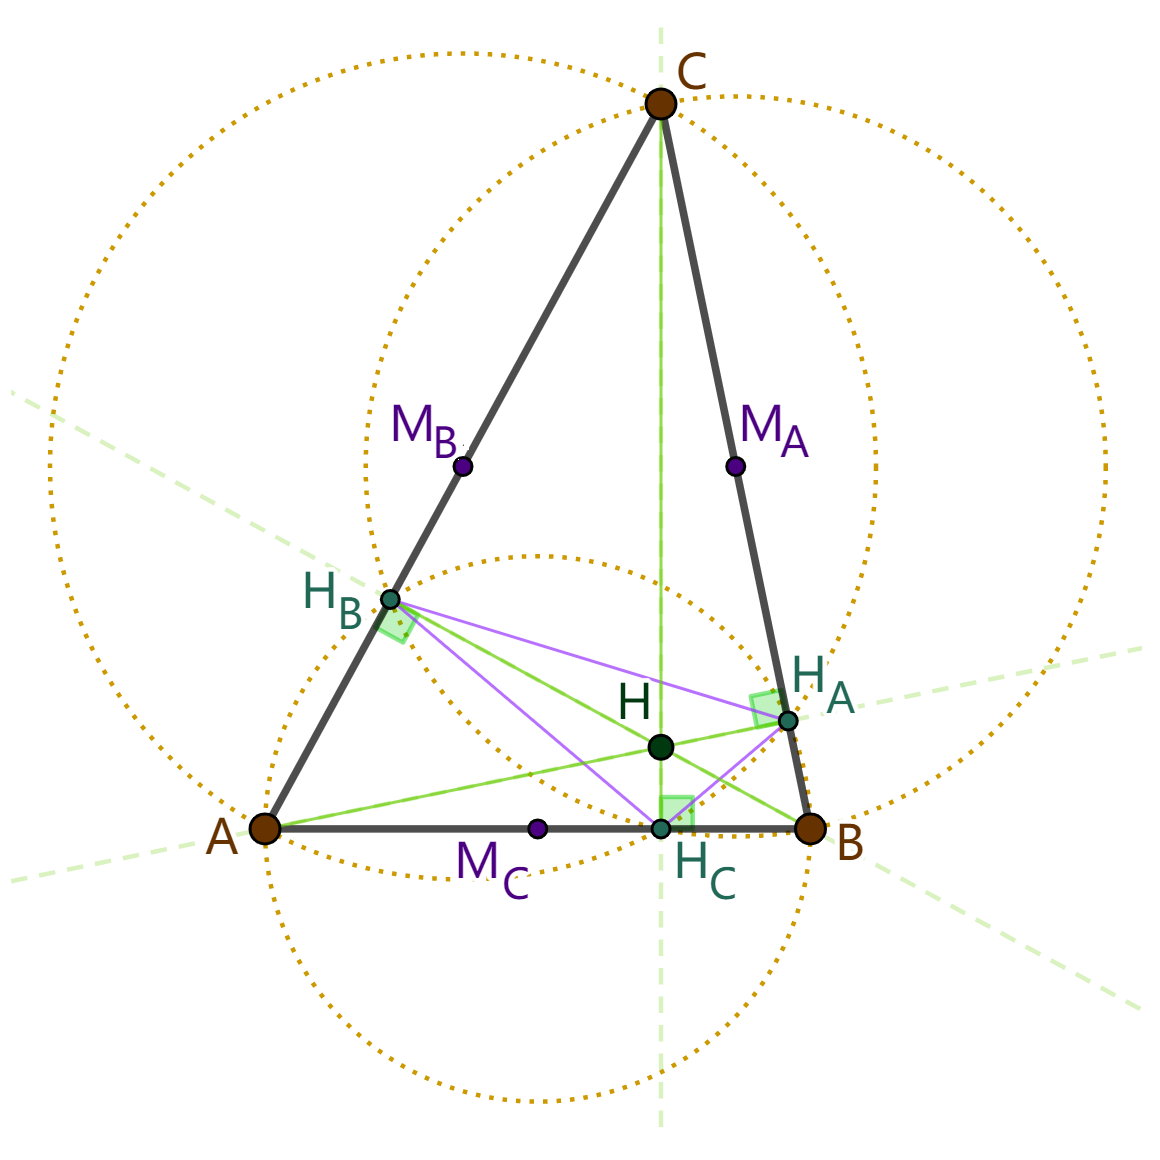
\includegraphics[width=0.48\textwidth]{垂心与外心1.png}
\end{wrapfigure}

考虑锐角三角形$ABC$,把顶点到对边的垂足分别记作$H_A, H_B, H_C$,垂心为$H$。
由于$\angle HH_AB = \angle BH_CH = 90^\circ$,两角之和为平角,故$H, H_A, H_C, B$四点共圆,
$\angle H_CHH_A + \angle H_ABH_C = 180^\circ$。这说明$\angle CHA = \angle H_CHH_A$是钝角,
$\triangle AHC$是钝角三角形。

考察钝角三角形$AHC$,它的顶点到对边的垂足也是$H_A, H_B, H_C$,而垂心是$B$。

类似地,我们可以证明$H, H_B, H_C, A$四点共圆,$H, H_A, H_B, C$四点共圆。
钝角三角形$BHC$、$CHA$的顶点到对边的垂足也是$H_A, H_B, H_C$,
而垂心分别是$A$和$B$。

于是,从锐角三角形$ABC$及其垂心$H$出发,可以得出四个三角形,每三个点构成的三角形的垂心,
是四个点中剩余的那个点。我们把这样的四点称为\textbf{垂心组}。

从钝角三角形及其垂心出发,一样可以得到一个垂心组。从直角三角形出发,其垂心和直角顶点重合,
四点的垂心组退化为三点。

从上面的讨论可知,垂心组四点共享三个垂足。任一顶点、垂心和另外两个顶点对应的垂足四点共圆。

考察$A, H_B, H_A, B$四点。由$\angle AH_BB = 90^\circ = \angle AH_AB$可知,
$A, H_B, H_A, B$四点共圆。由于$\angle AH_BB$是直角,$A, H_B, H_A, B$四点所在的圆,
圆心是边$AB$的中点$M_C$。同理,$A, H_C, H_A, C$四点共圆,圆心是边$AC$的中点$M_B$;
$B, H_C, H_B, C$四点共圆,圆心是边$BC$的中点$M_A$。

从$A, H_B, H_A, B$四点共圆可以推出:$\angle A = \angle CH_AH_B$,$\angle B = \angle H_AH_BC$。
也就是说,$\triangle CH_BH_A \backsim \triangle CBA$。

从以上两个四点共圆性质还可以推出$\angle HH_CH_A = \angle CAH$,$\angle HH_AH_C = \angle ACH$。
因此,$\triangle HH_AH_C \backsim \triangle HCA$。

以上是三角形垂心组的基本性质。垂心是顶点到对边垂线的交点。另外一个和边垂直的概念是边的中垂线。
如果把三角形的垂心和外心一起来看,会发现两者有密切的关联。

考虑锐角三角形$ABC$、其垂心$H$及其外心$O$。边$BC$可以看作$\triangle ABC$外接圆的弦。
圆心角$\angle BOC = 2\angle A$,因此在等腰三角形$BOC$中,
$$\angle CBO = 90^\circ - \frac{1}{2}\angle BOC = 90^\circ - \angle A = \angle HBA.$$
同理,$\angle BAO = \angle HAC$,$\angle ACO = \angle HCB$。

\begin{wrapfigure}[9]{r}{0.42\textwidth} %this figure will be at the right
    \vspace{-50pt}
    \flushright
    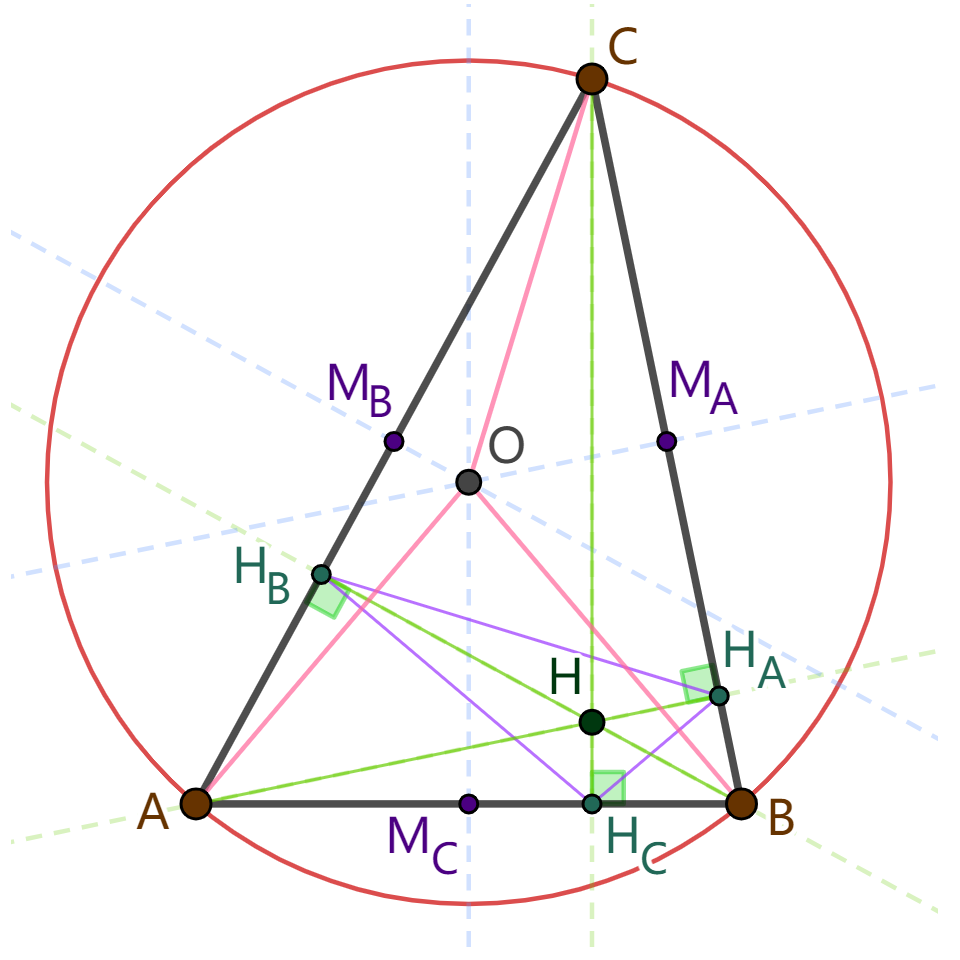
\includegraphics[width=0.4\textwidth]{垂心与外心2.png}
    % \caption*{\texttt{垂心和外接圆}}
\end{wrapfigure}

此外,$\angle H_CH_AB = \angle A$,因此$\angle H_CH_AB + \angle CBO = 90^\circ$。
这说明半径$OB \perp H_AH_C$。同理,半径$OA \perp H_BH_C$,$OC \perp H_AH_B$。

作点$A$在$ABC$外接圆上的对径点$A'$,$AA'$是直径,所以$\angle ACA'$是直角。因此
$$ \angle H_CHA' = 90^\circ - \angle ACH_C = \angle A.$$
另一方面,$A, H_B, H, H_C$四点共圆,所以
$$ \angle H_CHB = 180^\circ - \angle H_BHH_C = \angle A.$$
这说明$CA' \parallel HB$。
同理,我们可以得到$BA' \parallel HC$。因此四边形$A'BCH$是平行四边形。

作$B,C$的对径点$B', C'$,同样可以证明,
四边形$AB'HC$和$AHBC'$是平行四边形。

\begin{wrapfigure}[9]{r}{0.42\textwidth} %this figure will be at the right
    \vspace{-30pt}
    \flushright
    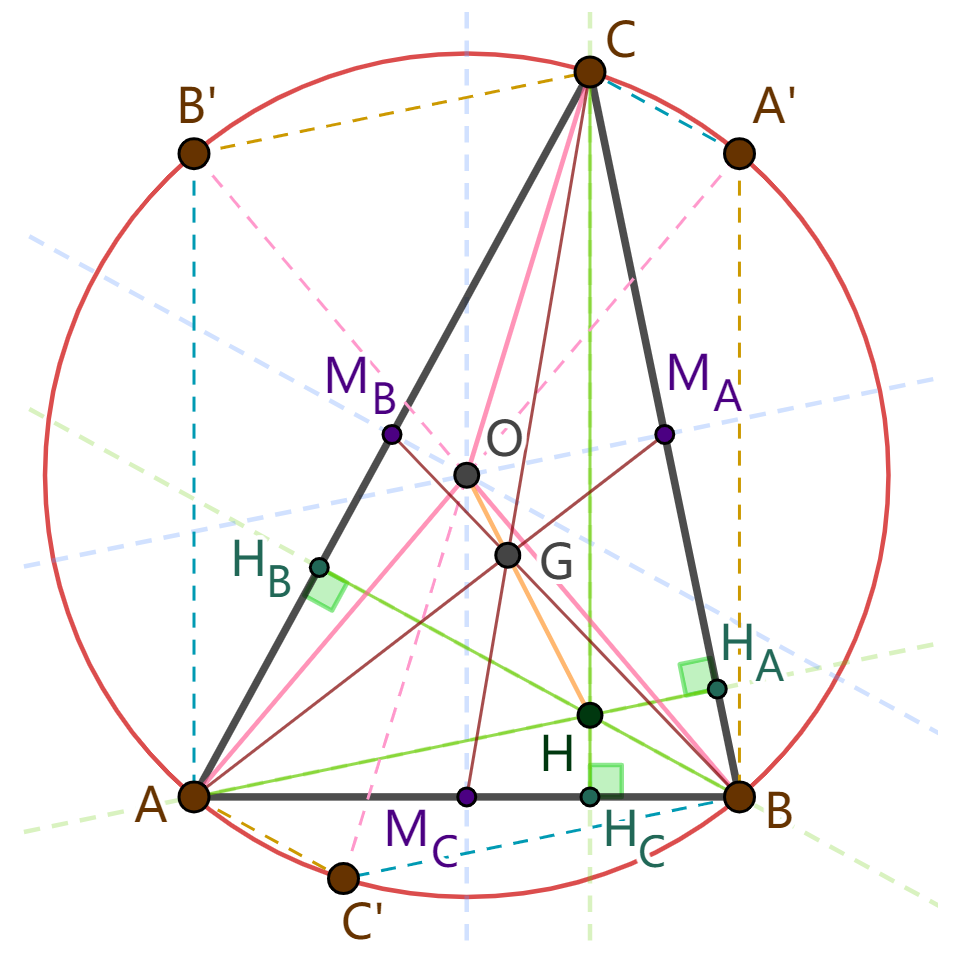
\includegraphics[width=0.4\textwidth]{垂心外心重心3.png}
    % \caption*{\texttt{垂心和外接圆}}
\end{wrapfigure}

连接圆心$O$和$AB$中点$M_C$,$O$是直径$AA'$的中点,所以$OM_C$平行于$A'B$,且长度为$A'B$一半。
我们把这种关系简称为“$OM_C$平行且等于$A'B$的一半”。

连接$OH$和$AM_C$。由于$OM_C$平行且等于$A'B$的一半,$A'B$平行且等于$HC$,
因此$OM_C$平行且等于$HC$的一半。记$OH$和$CM_C$交点为$G$,
不难看出,$\triangle OGM_C \sim \triangle GHC$,且
$$ \frac{|M_CG|}{|GC|} = \frac{|OG|}{|GH|} = \frac{|OM_C|}{|HC|} = \frac{1}{2}.$$
也就是说,点$G$在三角形$ABC$中线$CM_C$上,且到$C$点的距离是到$M_C$距离的两倍。
这说明$G$就是三角形$ABC$的重心。我们发现,三角形的垂心、外心和重心满足以下的性质:

\begin{tm}{\textbf{三心共线定理}}\label{tm:1-2-10}
    \mbox{} \\
    三角形$ABC$的垂心、外心和重心共线,重心位于外心和垂心为端点的线段上,
    而且重心到垂心的距离是重心到外心距离的两倍。
\end{tm}

\begin{xt}\label{xt:1-2-10}
    沿用本节记号,证明: \\\
    \indent 1. $|AH|\cdot |HH_A| = |BH|\cdot |HH_B| = |CH|\cdot |HH_C|.$\\
    \indent 2. $H$是$\triangle H_AH_BH_C$的内心。\\
    \indent 3. 记$\triangle ABC$的内心为$I$,旁心分别为$J_A, J_B, J_C$,则$I$是$\triangle J_AJ_BJ_C$的垂心。\\
    \indent 4. $H$关于$AB$的对称点$H^C$在$ABC$外接圆上,且$\widearc{AC'} = \widearc{H^CB}$。\\
    \indent 5. $\triangle AHB$、$\triangle AHC$和$\triangle CHB$的外接圆都和$\triangle ABC$的外接圆一样大。
    它们的圆心分别是$\triangle ABC$的外心$O$关于三边的对称点,和$O$组成垂心组。
    并且这个垂心组和垂心组$A,B,C,H$全等。
\end{xt}

\section{九点圆}

我们已经了解过三角形的外接圆、内切圆和旁切圆。本节我们再介绍三角形内部的一个特殊的圆。

设有三角形$ABC$,上一节中,我们证明了$\triangle ABC$的垂心$H$、外心$O$和重心$G$共线。
考虑线段$OH$,作它的中点$M$。我们知道$AHBC'$是平行四边形,所以$M_C$是其对角线$HC'$的中点。
因此,$MM_C$平行且等于$OC'$的一半。

作$CH$的中点$D_C$,由于$OM_C$平行且等于$CH$的一半,因此平行且等于$HD_C$。
也就是说,四边形$HD_COM_C$是平行四边形,于是$M_C, M, D_C$共线,$M$是$M_CD_C$的中点,
$|MD_C| = |MM_C| = \frac12 |M_CD_C|$。

$\triangle M_CH_CD_C$是直角三角形,所以斜边中点$M$到直角顶点$H_C$的距离是斜边长度$M_CD_C$的一半。
也就是说,
$$ |MD_C| = |MM_C| = |MH_C| = \frac12 |OC'| = \frac{\mathtt{R}}{2}.$$
其中$\mathtt{R}$是$ABC$的外接圆半径。

\begin{wrapfigure}[7]{r}{0.42\textwidth} %this figure will be at the right
    \vspace{-20pt}
    \flushright
    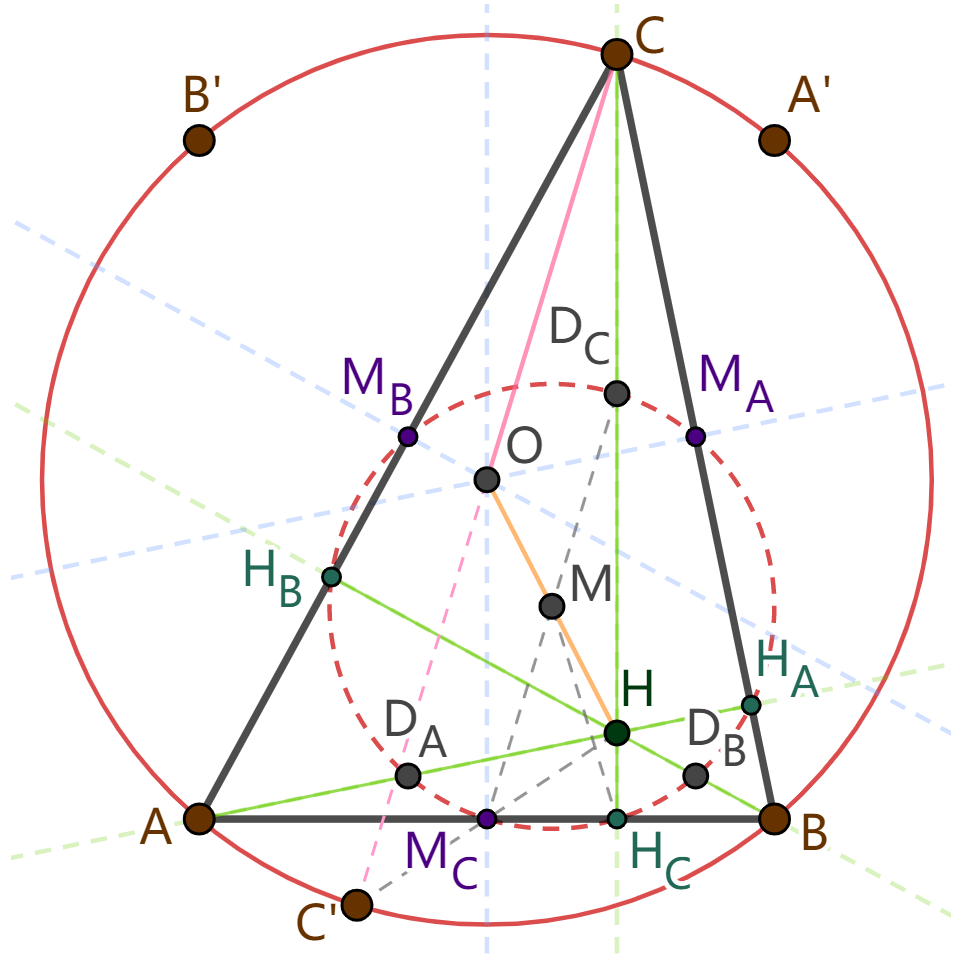
\includegraphics[width=0.4\textwidth]{九点圆1.png}
    % \caption*{\texttt{垂心和外接圆}}
\end{wrapfigure}

同理,我们也有
\begin{align}
    |MD_A| = |MM_A| = |MH_A| = \frac{\mathtt{R}}{2}, \notag \\
    |MD_B| = |MM_B| = |MH_B| = \frac{\mathtt{R}}{2} \notag 
\end{align} 
所以,以$M$为圆心,以$\frac{\mathtt{R}}{2}$为半径画圆,我们就会发现,这个圆经过三边中点,
三边上的垂足,以及三顶点到垂心连线的中点,合共九点。我们把这个圆称为\textbf{九点圆}。

\begin{tm}{\textbf{九点圆定理}}\label{tm:1-3-10}
    \mbox{} \\
    三角形三边中点、三边垂足,以及三顶点到垂心连线的中点共圆。
    圆心为外心与垂心的中点,半径为三角形外接圆半径的一半。
\end{tm}
三角形的九点圆的大小,刚好是三角形外接圆的一半。如果我们把三角形的垂心$H$看作“起点”,
那么三角形的外接圆可以看作是九点圆外延加倍得到的。比如,把线段$HD_C$加倍延长,就得到$HC$;
把线段$HM_C$加倍延长,就得到$HC'$;把线段$HH_C$加倍延长,就得到外接圆上一点$H^C$。
一般来说,从$H$出发,连接$H$和九点圆上任一点,加倍延长后,终点就会落在外接圆上。

\begin{xt}
    沿用本节记号,证明:\\
    \indent 1. 作外心$O$关于三边的对称点:$O_A, O_B, O_C$,则垂心$H$是$\triangle O_AO_BO_C$的外心。\\
    \indent 2. $\triangle O_AO_BO_C \simeq \triangle ABC$。两者关于点$M$对称,有共同的九点圆。\\
    \indent 3. 记$\triangle ABC$的旁心为$J_A, J_B, J_C$,则$\triangle J_AJ_BJ_C$的九点圆是$\triangle ABC$的外接圆。
\end{xt}

\section{圆内接多边形}
九点圆涉及了内接于同一个圆的九边形。对一般的多边形来说,成为圆内接多边形意味着什么呢?

从四边形的情况来看,顶点的位置顺序对形状很重要。如果顶点$A$、$B$、$C$、$D$按顺时针或逆时针顺序排列,
那么四边形$ABCD$是凸四边形,否则,四边形$ABCD$可能是凹四边形。

对一般的圆内接多边形,我们只研究最简单的一类:顶点按逆时针顺序排列的多边形。
具体来说,设圆$O$上有$n$个点:$A_1, A_2, \cdots , A_n$,从$A_1$出发构造圆映射$\gamma_{(O,A_1)}$,
把$[0, 360)$映射到圆周,那么$0$对应$A_1$。设$t_1, t_2, \cdots , t_n$分别对应$n$个点,
那么$0 = t_1 < t_2 < \cdots < t_n$。这样定义的圆内接多边形:$A_1A_2\cdots A_n$就是我们研究的对象。
这样定义的多边形,每个内角都在零角和平角之间。这样的多边形叫做\textbf{凸多边形}。

对于大于等于$3$的整数$n$,凸$n$边形$A_1A_2\cdots A_n$有$\frac{n(n-3)}{2}$条对角线。
具体来说,每个顶点和相邻两个顶点的连线是$n$边形的边,和其余$n-3$个顶点的连线是对角线。
因此每个点是$n-3$条对角线的端点。另一方面,每条对角线对应两个顶点,因此一共有$\frac{n(n-3)}{2}$条对角线。

凸多边形的内角和是否有规律呢?我们知道三角形的内角和是平角,凸四边形的内角和是两个平角
(或者说周角,如果把角度约定在负平角和正平角之间,则减去一个周角变成零角)。边数继续增多时,
我们定义凸$n$边形$A_1A_2\cdots A_n$的内角和为:

$$ \angle A_1A_2A_3 + \angle A_2A_3A_4 + \cdots + \angle A_{n-2}A_{n-1}A_{n} + \angle A_{n-1}A_{n}A_{1}+ \angle A_{n}A_{1}A_{2}$$

如果我们不把角度限定在负平角和正平角之间,可以猜测:凸$n$边形的内角和是$n-2$个平角。

如果凸多边形是圆内接多边形,我们可以这样证明:$n$个顶点把圆分为$n$段圆弧。每个顶点张成的内角,
对应了其中$n-2$段圆弧。如果考虑所有$n$个内角对应的圆弧,则每段圆弧计入$n-2$次(圆弧两端是内角顶点的时候不计入,
其它情况下都计入)。也就是说,$n$个内角和对应$n-2$个整圆。这些内角都是圆周角,
因此它们的和是$n-2$个整圆对应的圆周角,即$n-2$个平角。我们的猜想至少对圆内接多边形是正确的。

对一般凸多边形的情况,我们可以通过不断“裁剪”三角形来证明。我们还记得,凸四边形可以裁成两个三角形,
因此它的内角和是两个三角形的内角和。从另一个角度来看,我们通过裁掉一个三角形,把凸四边形变成了三角形。
对一般的凸$n$边形$A_1A_2\cdots A_n$来说,由于它的每个内角都介于零角和平角之间,我们可以考虑裁掉某个角,
把它变成$n-1$边形。比如,沿着线段$A_1A_3$剪一刀,
就把$A_1A_2\cdots A_n$分成了三角形$A_1A_2A_3$和$n-1$边形$A_1A_3\cdots A_n$。

\begin{tm}\label{tm:1-4-0}
    凸$n$边形的内角和是$n-2$个平角。
\end{tm}
\begin{proof}
    用归纳法证明。命题$P(n)$:凸$n+2$边形的内角和是$n$个平角。我们要证明$P(n)$对所有正整数$n$成立。\\
    $n=1$时,由于三角形内角和是平角,$P(1)$成立。\\
    假设$P(n)$成立,下面证明$P(n+1)$成立。\\
    设有凸$n+3$边形$A_1A_2A_3\cdots A_n$,将它裁成三角形$A_1A_2A_3$和$n-1$边形$A_1A_3\cdots A_n$。
    前者的内角和是平角。根据$P(n)$,后者的内角和是$n$个平角,因此,$A_1A_2A_3\cdots A_n$的内角和是$n+1$个平角。
    于是$P(n+1)$成立。\\
    因此对所有正整数$n$,命题$P(n)$成立。
\end{proof}

满足什么条件时,凸多边形是圆内接多边形呢?最直接的条件,自然是平面上有一个圆,
使多边形顶点都在圆上。或者说,能找到一点,到多边形各个顶点距离相等。

如果难以直接找到这样的点,可以查看多边形各边和各条对角线的垂直平分线。
如果多边形是圆内接多边形,它的边和对角线都是圆的弦,垂径定理说明其垂直平分线过圆心。
具体来说,可以考察两条边(或对角线)的垂直平分线的交点。这点如果到各个顶点距离相等,
那么多边形内接于以它为圆心的圆,否则多边形不是圆内接多边形。

有一种特殊的凸多边形必然是圆内接多边形:\textbf{正多边形}。
正多边形是各边等长,各内角相等的多边形。正三角形、正方形都是正多边形。
正多边形各个的内角角度是$\frac{180(n-2)}{n}^\circ$。

\begin{xt}\label{xt:1-4-0}
    \mbox{}\\
    \indent 1. 平行四边形、矩形、正方形、梯形、筝形,哪些总是圆内接多边形?哪些可以是圆内接多边形?要满足什么条件?\\
    \indent 2. 设有整数$1 \leqslant i,j,k,l \leqslant n$,圆内接$n$边形$A_1A_2\cdots A_n$中,$\angle A_iA_kA_j$和$\angle A_iA_lA_j$有什么关系?
\end{xt}

% \section{弧长和面积}
% 直观上,我们知道圆和圆弧的形状。我们已经学过,半径为$r$的圆,面积是$\pi r^2$,周长是$2\pi r$。
% 其中的$\pi$是常数,叫圆周率,大约等于$3.14$。在公理体系中,如何证明这一点呢?

% 这些知识看似不难,但要从基本的定义和公理出发,得到


\chapter{三角函数}
通过研究点、直线、角和三角形、四边形、圆形,我们对简单的平面图形有了更多的认识。
其中对三角形的研究贯通了我们对各种形状的探索。通过对三角形性质的理解,
我们建立了三角形和四边形、圆形乃至更复杂的形状之间的关系。

如果对前面学习的知识做一次整理,我们会发现,大多数的结论要么和共点、共线、共圆有关,
要么是长度之间、角度之间的相等或简单倍数关系。我们把这些结论称为定性结论。

在科学研究和生产实践中,我们更需要知道的是形状之间定量的关系。
比如,如果三角形的三边长度分别是$4,5,6$,我们希望知道三角形内角到底是多少度。
又比如,如果菱形两条邻边长度为$1$,夹角为$50^\circ$,我们希望知道菱形对角线的长度。
为此,我们从三角形的边角关系着手研究。

\begin{wrapfigure}[5]{r}{0.4\textwidth} %this figure will be at the right
    \vspace{-0pt}
    \flushright
    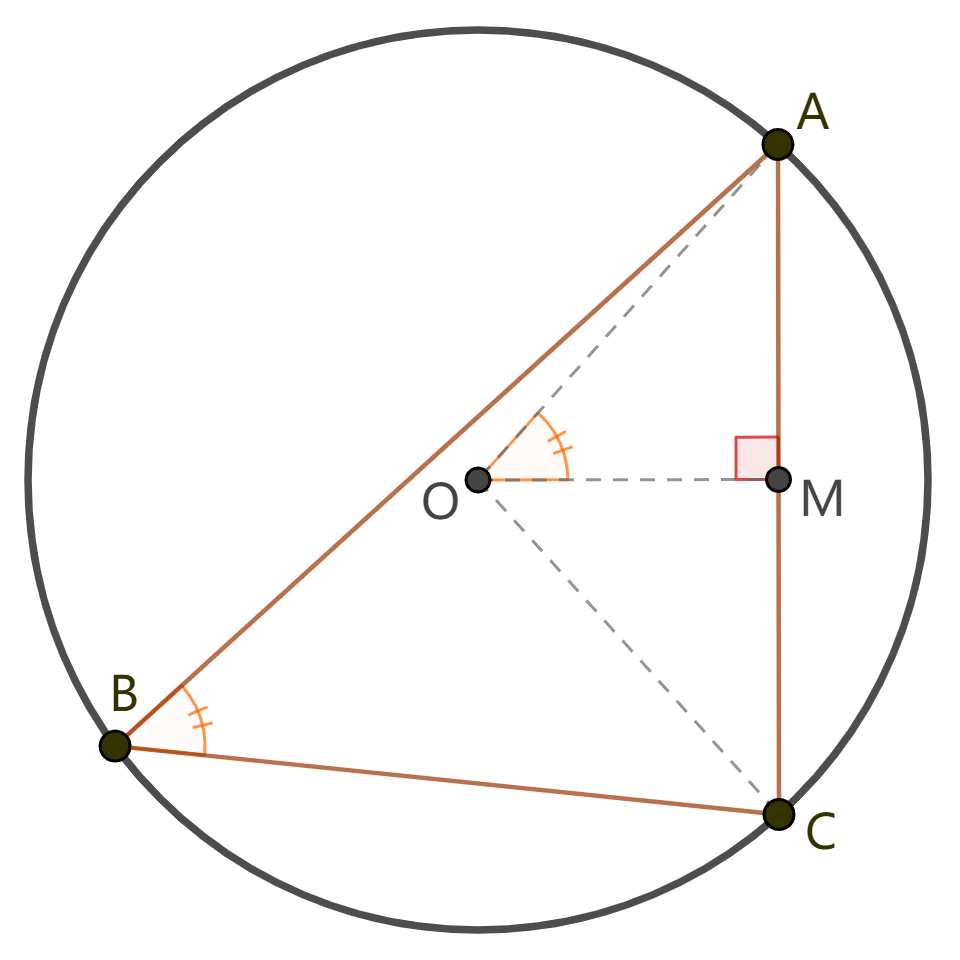
\includegraphics[width=0.36\textwidth]{三角函数1.png}
\end{wrapfigure}
我们的目标是解三角形:已知三角形部分边角的大小,求其余边角的值。

\section{正弦函数}
如右图,我们想知道三角形$ABC$中$\angle A$的角度和对边$BC$长度的关系。
为此,我们作$ABC$的外接圆$O$,则$BC$是$O$的弦。$\angle A$作为圆周角,
是圆心角$\angle COB$的一半。作$BC$中点$M$,则$\angle A = \angle MOB$。
这样,我们就把一般三角形的边角关系转化成了直角三角形$MBO$的边角关系。

那么,直角三角形的角和边有什么关系呢?我们先来看另一个问题。

考虑半径为$1$的圆$O$(这个圆以后会经常出现,我们把它叫做\textbf{单位圆})和圆上一点$S$。
给定角$\alpha$,以$OS$为始边,角的终边交圆$O$于点$P$。
称$\triangle SOP$为角$\alpha$对应的\textbf{单位三角形}(如下图)。
根据三角形面积公式(底乘高除以$2$),单位三角形的面积等于$P$到始边距离的一半。

\begin{figure}[H] %this figure will be at the right
    \vspace{4pt}
    \centering
    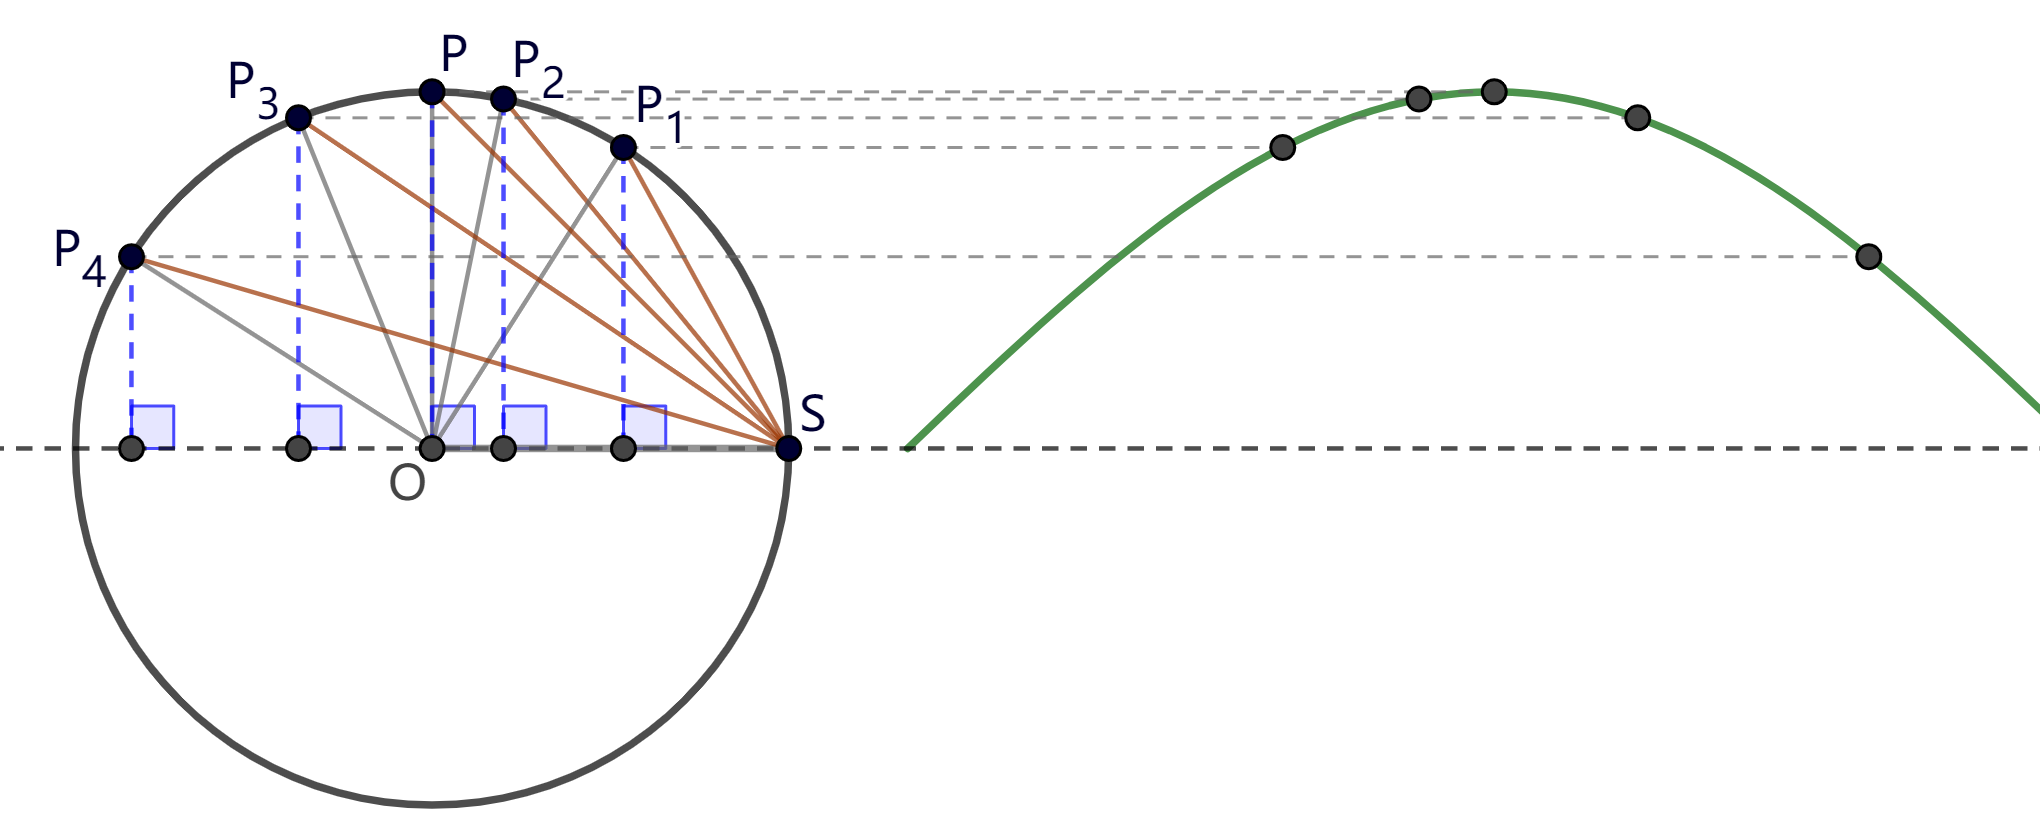
\includegraphics[width=0.8\textwidth]{三角函数2.png}
    % \caption*{\texttt{垂心和外接圆}}
\end{figure}

不难看出,$\alpha$为直角时,单位三角形的面积最大,为$\frac{1}{2}$。其它情况下,运用勾股定理可知,
$P$到始边距离小于半径,因此面积小于$\frac{1}{2}$。

我们把角$\alpha$对应的单位三角形的面积和直角对应的单位三角形面积之比称为$\alpha$的正弦或正弦值,
记为$\sin \alpha$。$\sin A$就是$P$到始边距离,也就是前面直角三角形$MBO$中$BM$与外接圆半径之比,
或弦长与外接圆直径之比。

角度在零角到平角之间的每个角,都可以按以上方法定义正弦。更准确来说,我们定义的是角度的正弦。不过,
它实际上对应着一个把数映射到数的映射,也就是函数。比如,$0$和$180$之间的任何实数,
都通过角度制的圆映射对应某个角度,从而对应某个正弦值。

另一种对应方法使用弧度,也就是把角度在单位圆上对应的弧长映射到角度的正弦值。
比如,$60^\circ$角对应着圆周的六分之一,
在单位圆上对应的弧长是$\frac{2\pi}{6} = \frac{\pi}{3}$。
我们就说$60^\circ$角的正弦值是$\sin \frac{\pi}{3}$。
把角度或角度在单位圆上的弧长对应到角度的正弦值的函数,称为\textbf{正弦函数}。

正弦函数有什么性质呢?观察不同角度对应的单位三角形可知,零角的正弦值是$0$(退化的三角形面积为$0$)。
从零角出发,随着角度增大,正弦值不断增大;直角时,正弦值达到最大值$1$。然后,随着角度增大,
正弦值不断减小;平角时,正弦值减为$0$。

两个角互为补角时,对应的单位三角形是同一个菱形按不同对角线剖开得到的一半。所以两者面积相等。
也就是说,\textbf{两个角互为补角,则正弦值相等}。因此,我们将把重点放在研究锐角的正弦值上。

\begin{figure}[H] %this figure will be at the right
    \vspace{4pt}
    \centering
    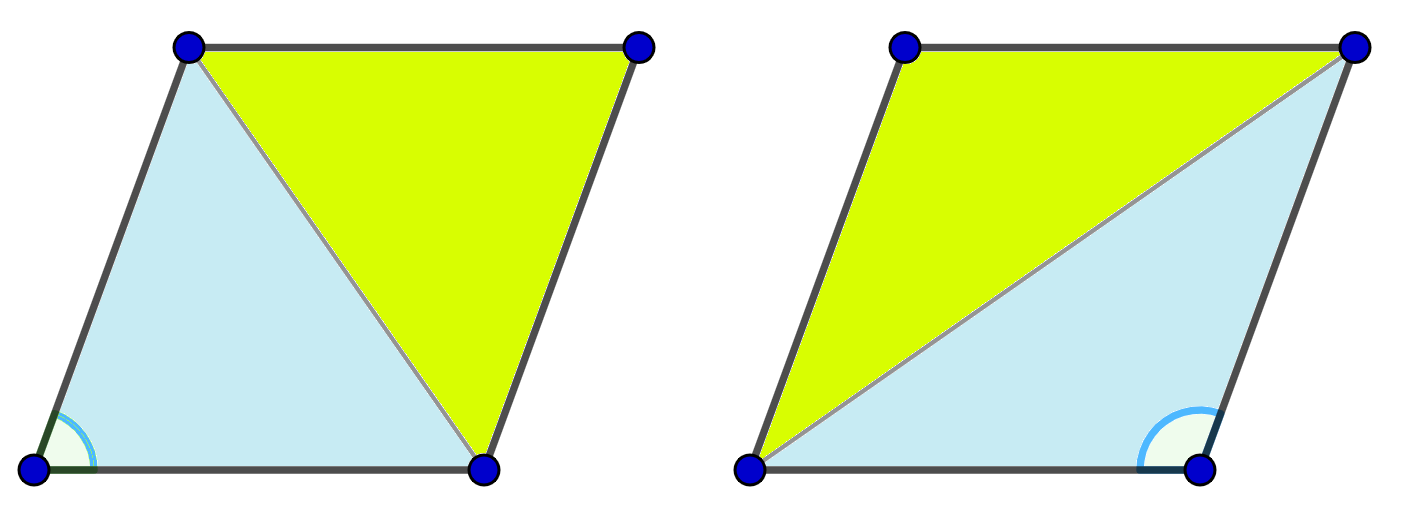
\includegraphics[width=0.5\textwidth]{正弦菱形1.png}
    % \caption*{\texttt{垂心和外接圆}}
\end{figure}

对具体的某个角度来说,怎么计算它的正弦值呢?这个问题不简单。以我们掌握的知识,
还无法精确计算任意角度的正弦值,甚至难以估计任意角度的正弦值。求解任意角度的正弦值属于实变函数分析的重要基础内容。
目前,我们可以使用正弦函数表,查找角度的正弦值,或通过使用计算器、编程等方式,
借助计算机计算角度的正弦值。使用正弦表,可以方便地查找角度对应的正弦值。以下是整数角度的正弦表:

% 正弦表
\begin{center}
    \begin{tabular}{| p{1em}<{\centering} | p{2.4em}<{\centering} | p{2.4em}<{\centering} | p{2.4em}<{\centering} | p{2.4em}<{\centering} | p{2.4em}<{\centering} | p{2.4em}<{\centering} | p{2.4em}<{\centering} | p{2.4em}<{\centering} | p{2.4em}<{\centering} |}
        \hline
                  & $0^\circ$& $10^\circ$ & $20^\circ$ & $30^\circ$ & $40^\circ$ & $50^\circ$ & $60^\circ$ & $70^\circ$ & $80^\circ$ \\ [0.5ex] 
        \hline
        $0^\circ$ & $0.0000$ &  $0.1736$  &  $0.3420$  &  $0.5000$  &  $0.6428$  &  $0.7660$  &  $0.8660$  &  $0.9397$  &  $0.9848$  \\
        \hline
        $1^\circ$ & $0.0175$ &  $0.1908$  &  $0.3584$  &  $0.5150$  &  $0.6561$  &  $0.7771$  &  $0.8746$  &  $0.9455$  &  $0.9877$  \\
        \hline
        $2^\circ$ & $0.0349$ &  $0.2079$  &  $0.3746$  &  $0.5299$  &  $0.6691$  &  $0.7880$  &  $0.8829$  &  $0.9511$  &  $0.9903$  \\
        \hline
        $3^\circ$ & $0.0523$ &  $0.2250$  &  $0.3907$  &  $0.5446$  &  $0.6820$  &  $0.7986$  &  $0.8910$  &  $0.9563$  &  $0.9925$  \\
        \hline
        $4^\circ$ & $0.0698$ &  $0.2419$  &  $0.4067$  &  $0.5592$  &  $0.6947$  &  $0.8090$  &  $0.8988$  &  $0.9613$  &  $0.9945$  \\
        \hline
        $5^\circ$ & $0.0872$ &  $0.2588$  &  $0.4226$  &  $0.5736$  &  $0.7071$  &  $0.8192$  &  $0.9063$  &  $0.9659$  &  $0.9962$  \\
        \hline
        $6^\circ$ & $0.1045$ &  $0.2756$  &  $0.4384$  &  $0.5878$  &  $0.7193$  &  $0.8290$  &  $0.9135$  &  $0.9703$  &  $0.9976$  \\
        \hline
        $7^\circ$ & $0.1219$ &  $0.2924$  &  $0.4540$  &  $0.6018$  &  $0.7314$  &  $0.8387$  &  $0.9205$  &  $0.9744$  &  $0.9986$  \\
        \hline
        $8^\circ$ & $0.1392$ &  $0.3090$  &  $0.4695$  &  $0.6157$  &  $0.7431$  &  $0.8480$  &  $0.9272$  &  $0.9781$  &  $0.9994$  \\
        \hline
        $9^\circ$ & $0.1564$ &  $0.3256$  &  $0.4848$  &  $0.6293$  &  $0.7547$  &  $0.8572$  &  $0.9336$  &  $0.9816$  &  $0.9998$  \\
        \hline
    \end{tabular}
\end{center}
每列的数据十位相同,每行的数据个位相同。比如,要查$26^\circ$的正弦值,就在十位为$2$的第三列,找到个位为$6$的
第七行,查得正弦值为$0.4384$。

对于非整数角度的正弦值,我们可以查询更精确的正弦表,或者用一次函数来近似估计。
如果我们把整数角度的正弦值看作正弦函数的函数值,在直角坐标系上画出函数值对应的点,
可以观察到正弦函数的值从$0$平稳增长到$1$。因此,可以认为两个整数角度之间,
正弦函数的图像近似于线段,也就是一次函数图像的一部分。因此,非整数角度的正弦值可以通过计算线段上点的坐标而得到。

举例来说,$37^\circ$和$38^\circ$之间的角度(比如说$37.3^\circ$)的正弦值,
可以看作经过$(37, \sin 37^\circ)$和$(38, \sin 38^\circ)$两点的一次函数图像在横坐标为$37.3$时对应的纵坐标。
这个一次函数可以写成:

$$ y = \sin 37^\circ + \frac{\sin 38^\circ - \sin 37^\circ}{38 - 37} \cdot (x - 37)$$

横坐标$x=37.3$时,代入函数表达式,就得到:
\begin{align}
    y &= \sin 37^\circ + 0.3\cdot(\sin 38^\circ - \sin 37^\circ ) \notag \\
    &= 0.6018 + 0.3 \cdot (0.6157 - 0.6018) \approx 0.60597 \notag
\end{align}
实际上$\sin 37.3^\circ \approx 0.60599$,可见偏差不大。

反过来,如果已知角的正弦值,也可以通过查表,估计角度的大小。比如,已知$\sin A = 0.83$,
查表可知$\angle A$大小在$56^\circ$和$57^\circ$之间。

\begin{wrapfigure}[5]{r}{0.42\textwidth} %this figure will be at the right
    \vspace{-25pt}
    \flushright
    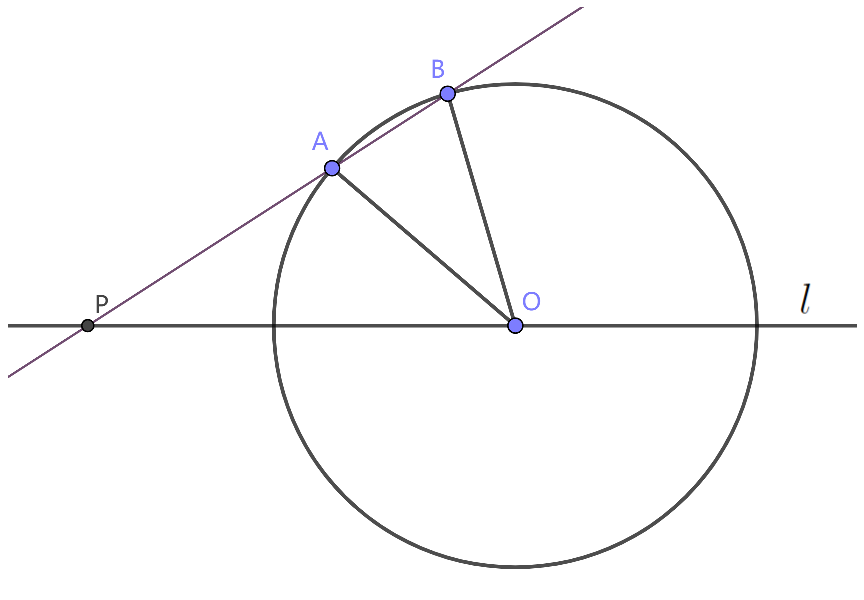
\includegraphics[width=0.4\textwidth]{正弦习题1.png}
\end{wrapfigure}

想一想,如果要得到更精确的结果,
除了查询更精确的正弦表,还可以怎么做?

\begin{xt}
    如右图,延长$BA$交$l$于点$P$。\\
    \indent 1. 计算$S_{\triangle AOP}$和$S_{\triangle BOP}$。 \\
    \indent 2. 通过比较$S_{\triangle AOP}$和$S_{\triangle BOP}$,证明锐角的正弦值随角度增大而增大,
    钝角的正弦值随角度增大而减小。 \\
    \indent 3. 从$46^\circ$、$48^\circ$的正弦值出发,用一次函数近似估计$47^\circ$,
    和正弦表上的值比较。哪个值比较大?对别的角度试一试,估计值的偏差有什么规律? \\
    \indent 4. 已知某锐角的正弦值为$0.73$,请估计它的角度大小。
\end{xt}

\section{正弦定理}

我们可以用正弦值来探讨三角形的边角关系。首先把正弦值应用到一般三角形的面积上。
我们知道$\angle A$对应的单位三角形的面积是$\frac{1}{2}\sin A$。
如果$\angle A$的两邻边长度分别是$b$和$c$,那么根据等高三角形的面积关系,
三角形的面积是单位三角形的$bc$倍,也就是$\frac{1}{2}bc\sin A$。

定理:三角形两边长度为$b$和$c$,夹角为$A$,则面积为$\frac{1}{2}bc\sin A$。

设三角形$ABC$中$A,B,C$对边长度为$a,b,c$,那么它的面积可以用三种方式表示:
$$ S_{\triangle ABC} = \frac{1}{2}ab\sin C = \frac{1}{2}ca\sin B = \frac{1}{2}bc\sin A.$$
两边除以$\frac{abc}{2}$,就得到:
$$  \frac{2S_{\triangle ABC}}{abc} = \frac{\sin C}{c} = \frac{\sin B}{b} = \frac{\sin A}{a}. $$

\begin{wrapfigure}[8]{r}{0.4\textwidth} %this figure will be at the right
    \vspace{-30pt}
    \flushright
    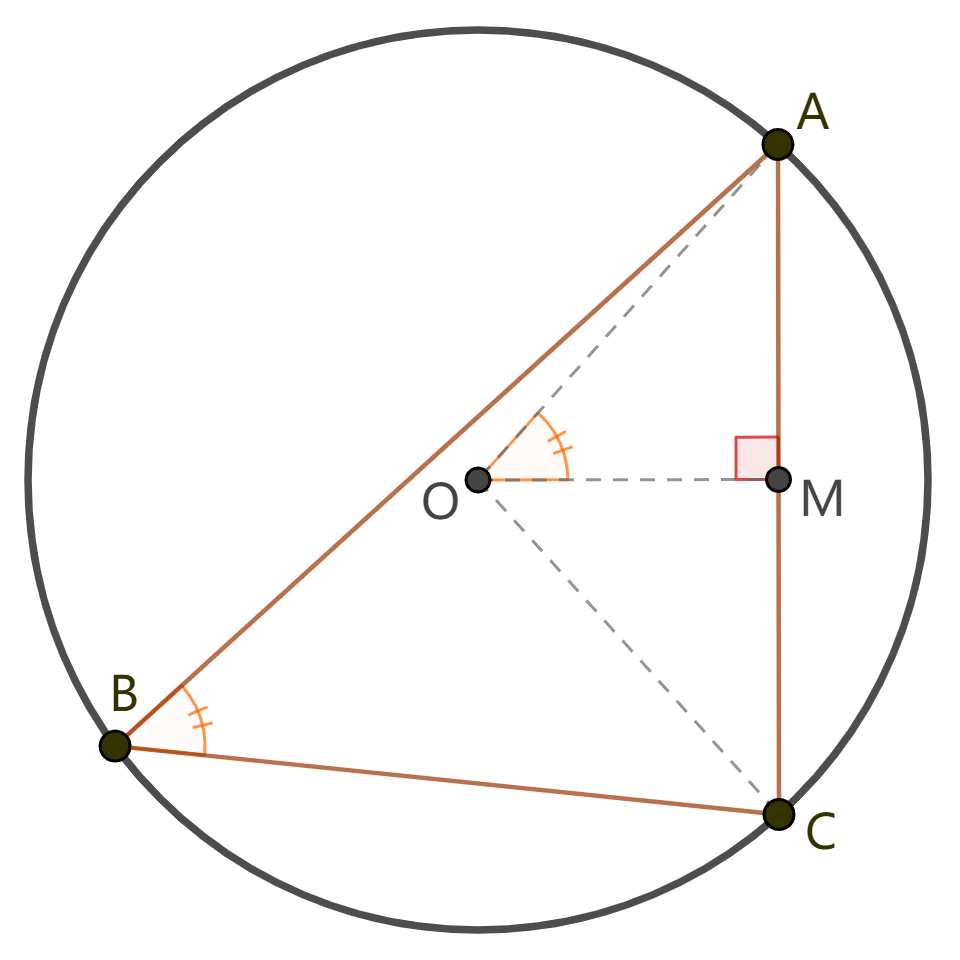
\includegraphics[width=0.36\textwidth]{三角函数1.png}
\end{wrapfigure}

上式告诉我们,三角形三个内角的正弦值和对边长度的比是定值$\frac{2S_{\triangle ABC}}{abc}$。
如何理解这个定值呢?让我们回到前面的三角形$MOB$。
我们知道$BM = \mathtt{R}\sin A$,其中$\mathtt{R}$是$\triangle ABC$外接圆半径。
所以$ \frac{a}{2} = \mathtt{R}\sin A$,即$ \frac{\sin A}{a} = \frac{1}{2\mathtt{R}}$。也就是说,
$$ \frac{a}{\sin A} = \frac{b}{\sin B} = \frac{c}{\sin C} =  2\mathtt{R}. $$

\begin{tm}{\textbf{正弦定理} }\label{tm:2-1-10}
    三角形任一边长与其对角正弦值之比为外接圆直径。
\end{tm}
从正弦定理可以立刻得出:三角形的面积等于三边长之积与外接圆半径之比的四分之一。
$$S_{\triangle ABC} = \frac{abc}{4\mathtt{R}}. $$ 

下面来看正弦定理的具体应用。

\begin{ex}\label{ex:2-1-10}
    三角形$ABC$中,边$AB$、$AC$长度分别为$3$和$5$,$\angle B = 80^\circ$,求$BC$的长度和$\angle C$的大小。    
\end{ex}
\begin{so}
    根据正弦定理:
    $$ \frac{|AC|}{\sin B} = \frac{|AB|}{\sin C},$$
    所以$\sin C = \frac{|AB|\sin B}{|AC|}$。
    查表知$\sin 80^\circ = 0.9848$,算得$\sin C \approx 0.5909$,
    反查正弦表可知$\angle C \approx 36.2^\circ$或$\angle C \approx 143.8^\circ$。
    由于三角形内角和是平角,$\angle C + \angle B < 180^\circ$,故排除$\angle C \approx 143.8^\circ$。
    于是$\angle C \approx 36.2^\circ$,$\angle A = 180^\circ - \angle B - \angle C \approx 63.8^\circ$,
    使用正弦定理可算得:
    $$ |BC| = \frac{|AB|\sin A}{\sin B} = \frac{3 \cdot \sin 80^\circ}{\sin 63.8^\circ} \approx 3.29 $$
\end{so}

已知三角形两边长度和其中一边对角的大小,可以根据正弦定理得出另一边对角的正弦值,从而得出它的角度。
用平角减去两角角度,就得到第三个角的大小。再次使用正弦定理,就得到第三边的长度。要注意的是,
用正弦定理算出的是角的正弦值,而不是角度。由于互为补角的正弦值相等,同一个正弦值对应两个互为补角的角度。
因此,给定三角形两边和其中一边的对角,并不一定能确定三角形的形状。换句话说,“边边角”不能用来证明三角形全等。

\begin{ex}\label{ex:2-1-20}
    已知三角形$ABC$中,$\angle A = 64^\circ$,$\angle B = 75^\circ$,$\angle C$对边长度$c=4$,求另两边的长度。
\end{ex}
\begin{so}
    三角形内角和为平角,所以$\angle C = 180^\circ - \angle A - \angle B = 41^\circ$。根据正弦定理:
    $$ \frac{a}{\sin 64^\circ} = \frac{b}{\sin 75^\circ} = \frac{c}{\sin 41^\circ}.$$
    所以$a = \frac{c \sin 64^\circ}{\sin 41^\circ} = \frac{4 \times 0.8988}{0.6561} \approx 5.48 $,$b = \frac{c \sin 75^\circ}{\sin 41^\circ} = \frac{4 \times 0.9659}{0.6561} \approx 5.89 $。
\end{so}

已知两内角大小和一边的长度,等于知道所有内角大小和一边边长。根据正弦定理,可以算出另两边的长度。
这说明“角边角”和“角角边”都可以用来证明三角形全等。

正弦定理不仅可以用来处理定量关系,也可以用来处理定性关系。三角形的边长和对角的正弦值之比是定值,
所以,边长越大,对角的正弦值也越大。而锐角的正弦值随着角度增大而增大,至直角达到最大。
所以,锐角和直角三角形中,较大的边,对角也较大,较大的角,对边也较大。
这个性质称为“\textbf{大边对大角}”、“\textbf{大角对大边}”。

对钝角三角形,“大边对大角”、“大角对大边”的结论是否也成立呢?
设三角形$ABC$中$\angle A$是钝角,则$\angle A$的补角是锐角。
三角形内角和为平角,所以$180^\circ - \angle A = \angle B + \angle C > \angle B$,
$\angle A$的补角大于$\angle B$,即$\sin A = \sin (B + C) > \sin B$。
同理,$\sin A > \sin C$。钝角$\angle A$作为较大的角,
其正弦值大于锐角$\angle B$和$\angle C$。
而$\angle B$和$\angle C$同为锐角,“大边对大角”、“大角对大边”的结论在两者之间同样成立。
综上所述,任意三角形中,“大边对大角”、“大角对大边”的结论总成立。

\begin{xt}\label{xt:2-1-10}
    \mbox{} \\
    \indent 1. 设三角形$ABC$内角$A,B$的公共边为$c$,证明:$S_{\triangle ABC} = \frac{c^2\sin A\sin B}{\sin (A+B)}$。 \\
    \indent 2. 三角形一边的长度是另一边的$2$倍。证明:至少有一个内角不大于$30^\circ$,一个内角不小于$75^\circ$。 \\
    \indent 3. 已知三角形$ABC$中$\angle A = 36^\circ$,$\angle B = 60^\circ$,$\angle C$对边长度$c = 8$,求另两边的长度。 \\
    \indent 4. 已知三角形两边长度是$4$、$5$,一个内角是$40^\circ$,第三边的长度有几种可能?找出所有满足条件的三角形。 \\
    \indent 5. 已知三角形两边长度是$4$、$5$,一个内角是$70^\circ$,第三边的长度有几种可能?结论和上一题有什么不同?找出所有满足条件的三角形。
\end{xt}


\section{余弦函数}
\begin{ex}\label{ex:2-2-10}
    \mbox{} \\
    \indent 1. 三角形$ABC$中,边$BC$、$AC$的长度分别是$4$、$6$,$\angle C = 50^\circ$,求$AB$长度。\\
    \indent 2. 三角形$ABC$中,边$AB$、$AC$、$BC$的长度分别为$3$、$5$、$6$,求三个内角的大小。
\end{ex}
使用正弦定理,我们列出以下等式:\\
\indent 1. $ \frac{4}{\sin A} = \frac{6}{\sin B} = \frac{|BC|}{\sin 50^\circ}.$ \\
\indent 2. $ \frac{6}{\sin A} = \frac{5}{\sin B} = \frac{3}{\sin C}.$

每个等式中都有两个未知量。我们无法直接用正弦定理计算内角的正弦值了。
不过,既然我们能通过“边边边”和“边角边”证明三角形全等,这让我们猜想,有别的方法计算内角的角度。

第一题中,让我们把$\angle C$改为直角,那么根据勾股定理,$|AB| = \sqrt{4^2+6^2} = 2\sqrt{13}$。

第二题中,让我们把$AB$、$AC$、$BC$的长度换成$3$、$4$、$5$,我们观察到最长边边长的平方等于另两边边长的平方和。
根据勾股定理逆定理,三角形是直角三角形。所以$\angle A$是直角。
用正弦定理解得$\sin B = 0.8$,$\sin C = 0.6$,查表可知$\angle B \approx 53^\circ$,
$\angle C \approx 37^\circ$。

可以看出,对于直角三角形,由于有勾股定理作为“武器”,我们总可以破解三角形的边角关系。
因此,我们需要“升级装备”,把勾股定理推广为对一般的三角形也适用的结论。
为此,我们需要定义角的余弦。

什么是角的余弦呢?我们已经定义了角的正弦。在直角三角形中,锐角的正弦是对边长度与斜边长度之比。
这个公式中我们用到了三角形的两条边。我们定义锐角的\textbf{余弦}(或\textbf{余弦值})
为剩余的直角边(也就是相邻的直角边)长度与斜边长度之比。在$MOB$的例子中,
角$A$的余弦就是弦$BC$的弦心距,记为$\cos A$。

显然,直角三角形中,一个锐角的邻边就是另一个锐角的对边。所以\textbf{锐角的余弦等于它的余角的正弦}:
$$ \forall \,\, 0 \leqslant A \leqslant 90^\circ, \,\,\, \cos A = \sin (90^\circ - A). $$
这样我们就定义了\textbf{余弦函数}。零角的余弦是$1$。从零角出发,随着角度增大,角的余弦逐渐减小。
直角时,余弦值达到最小值$0$。

此外,角的正弦和余弦分别是直角三角形两条直角边和斜边的比值。所以根据勾股定理,
$$ \cos^2 A + \sin^2 A = 1.$$
其中$\cos^2 A, \sin^2 A$分别是$(\cos A)^2, (\sin A)^2$的简便记法。这个结论也叫\textbf{三角勾股定理}。

怎么计算角的余弦值呢?从三角勾股定理定理可以看出,已知锐角的正弦,就可以得到它的余弦:
$\cos A = \sqrt{1 - \sin^2 A}$。所以,可以查正弦表得到角的正弦值,再求出余弦值。
反过来,已知锐角的余弦,可以先算出它的正弦,然后查表得到角度。

\begin{xt}
    \mbox{} \\
    \indent 1. 从等腰直角三角形的性质出发,计算$45^\circ$的正弦和余弦值。 \\
    直角三角形$ABC$中,$\angle C$是直角。斜边长度$c$是直角边长度$a$的$2$倍。 \\
    \indent 2. 作斜边中点$M$,证明:$\triangle BMC$是正三角形。 \\
    \indent 3. 计算$30^\circ$和$60^\circ$的正弦和余弦值。 \\
    等腰三角形$ABC$中,顶角$\angle A$是底角$\angle B$的$2$倍。 \\
    \indent 4. 设$\angle B$的平分线交对边于点$D$。证明:$\triangle ABC \sim \triangle BCD$。 \\
    \indent 5. 设底边长$a = 1$,腰长$b = c = x$,证明:$x^2 - x - 1 = 0$。 \\
    \indent 6. 计算$18^\circ$、$36^\circ$、$54^\circ$和$72^\circ$的正弦和余弦值。
\end{xt}

\section{余弦定理}

定义了角的余弦,我们再来看前面“边边边”的问题(例题\ref{ex:2-2-10}第一题)。
如果$\angle C$是直角,那么根据勾股定理,可以直接求出$AB$长度。如果$\angle C$不是直角,
我们希望把问题转化为直角三角形的边角关系。

作顶点$A$到$BC$的高,记垂足为$H_A$,则$H_A \neq C$。$\triangle ACH_A$是直角三角形,
所以$|AH_A| = |AC|\sin C = b\sin C$。如果$\angle C$是锐角,那么$H_A$在线段$BC$上,
$|CH_A| = |AC|\cos C = b\cos C$;如果$\angle C$是钝角,那么$H_A$在线段$BC$延长线上,
$|CH_A| = |AC|\cos C = b\cos (180^\circ - C)$。

\begin{figure}[H] %this figure will be at the right
    \vspace{4pt}
    \centering
    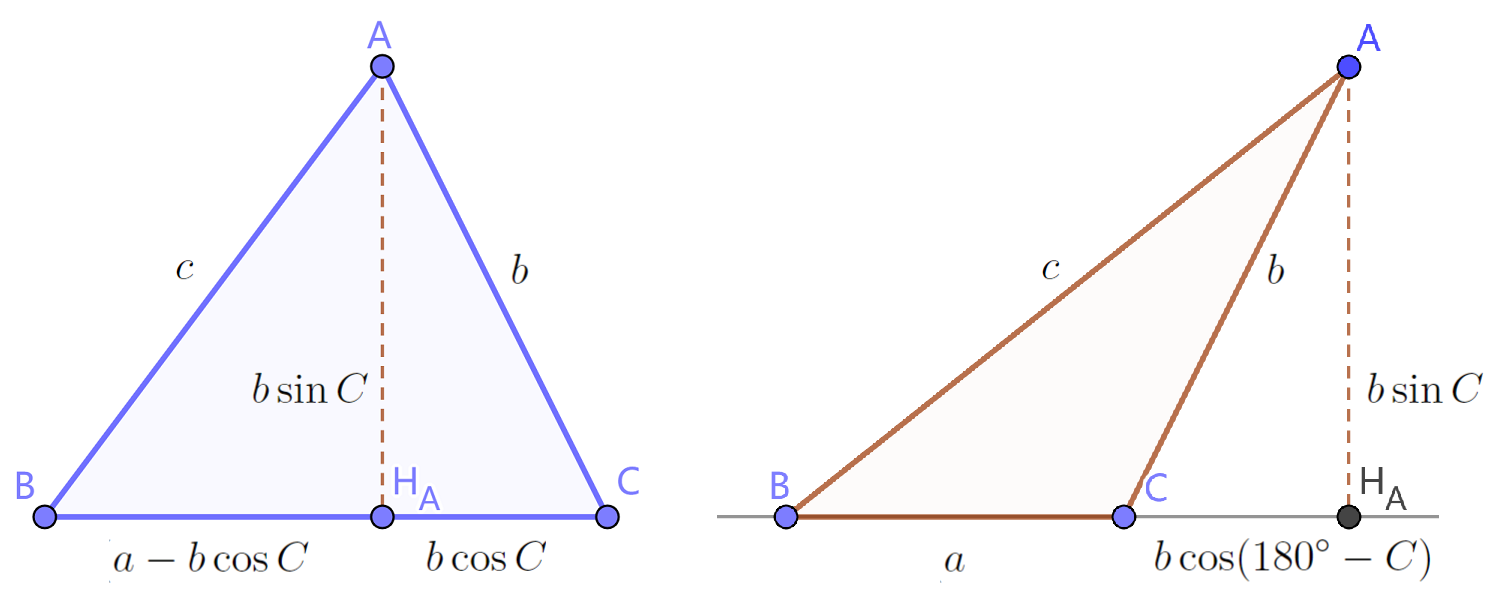
\includegraphics[width=0.8\textwidth]{余弦定理1.png}
    % \caption*{\texttt{垂心和外接圆}}
\end{figure}

$\triangle ABH_A$是直角三角形。根据勾股定理,$|AB|^2 = |AH_A|^2 + |BH_A|^2 $。
如果$\angle C$是锐角,那么
$$ |AB|^2 = |AH_A|^2 + |BH_A|^2 = |AH_A|^2 + (|BC| - |CH_A|)^2$$
即
\begin{align}
    c^2 &= (b\sin C)^2 + (a - b\cos C)^2 \notag \\
    &= b^2\sin^2 C + b^2\cos^2 C + a^2 - 2ab\cos C \notag \\
    &= a^2 + b^2 - 2ab\cos C \notag
\end{align}

我们得到了$a$、$b$、$c$和$\angle C$的关系。这个关系叫做\textbf{余弦定理}。
可以看出,$\angle C$为直角时,余弦定理就变成了勾股定理。所以,余弦定理是勾股定理的“升级版本”,
勾股定理可以看作是余弦定理的特例。
使用余弦定理,我们可以解决例题\ref{ex:2-2-10}第一题。
\begin{so}
    根据余弦定理,
    $$c^2 = a^2 + b^2 - 2ab \cos C = 4^2 + 6^2 - 2\cdot 4\cdot 6 \cos 50^\circ \approx 21.15.$$
    因此$c \approx \sqrt{21.15} \approx 4.6$。
\end{so}
用同样的方法,能否解决第二题呢?我们列出等式:
$$6^2 = 3^2 + 5^2 - 2 \cdot 3\cdot 5 \cos C $$
解得$\cos C = -\frac{1}{15}$。显然,任何锐角或直角的余弦都不是负数。我们猜测,这是因为$C$是钝角,
而前面的推导中,$\angle C$是锐角。

来看$\angle C$是钝角的情况。如果$\angle C$是钝角,那么
$$ |AB|^2 = |AH_A|^2 + |BH_A|^2 = |AH_A|^2 + (|BC| + |CH_A|)^2$$
即
\begin{align}
    c^2 &= (b\sin C)^2 + (a + b\cos (180^\circ - C))^2 \notag \\
    &= b^2\sin^2 C + b^2\cos^2 (180^\circ - C) + a^2 + 2ab\cos (180^\circ - C) \notag
\end{align}

可以看到,对钝角三角形,余弦定理的表达式比锐角三角形复杂很多。
把$a=3$、$b=5$、$c=6$代入钝角的余弦定理公式,我们发现难以解出$C$。
公式中,含有$C$的项无法像锐角的情况里那样合并化简,原因在于我们没有定义钝角的余弦值,
只能用锐角$180^\circ - C$的余弦值来表示。

如何定义钝角的余弦值呢?钝角的正弦为其补角的正弦。我们希望钝角的余弦也满足三角勾股定理:
$$ \sin^2 C +  \cos^2 C = 1 $$
这就要求
\begin{align}
    \cos C &= \sqrt{1 - \sin^2 C} \notag \\
    &= \sqrt{1 - \sin^2 (180^\circ - C)} \notag \\
    &= \pm\cos (180^\circ - C) \notag
\end{align}

如果我们定义钝角的余弦为它补角的余弦:$ \cos C = \cos (180^\circ - C)$,钝角三角形的余弦定理就变成:
$$ c^2 = a^2 + b^2 + 2ab \cos C.$$
如果我们定义钝角的余弦为它补角的余弦的相反数:$ \cos C = -\cos (180^\circ - C)$,钝角三角形的余弦定理就变成:
$$ c^2 = a^2 + b^2 - 2ab \cos C.$$
显然,后一种情况下,钝角三角形和锐角三角形余弦定理的形式就统一了。接下来我们会看到,后者在各个方面都更加合理。

\begin{xt}
    \mbox{}\\
    \indent 1. 已知三角形三边长为$5$、$7$、$8$,求三内角的大小。\\
    $\triangle ABC$中,$|AB|=6,|BC|=3,|CA|=5$,\\
    \indent 2. 求$\angle A$的大小。\\
    \indent 3. 求$\angle B, \angle C$的大小。
\end{xt}

\section{和差角公式}

解决平面形状的问题时,我们常常需要处理角度的和与差。给定两个角度$\alpha$、$\beta$,
我们希望能够给出$\alpha + \beta$、$\alpha - \beta$的正弦和余弦值。换句话说,
我们希望能够打通正弦函数、余弦函数和实数的加减法的关系。

\begin{figure}[H] %this figure will be at the right
    \vspace{4pt}
    \centering
    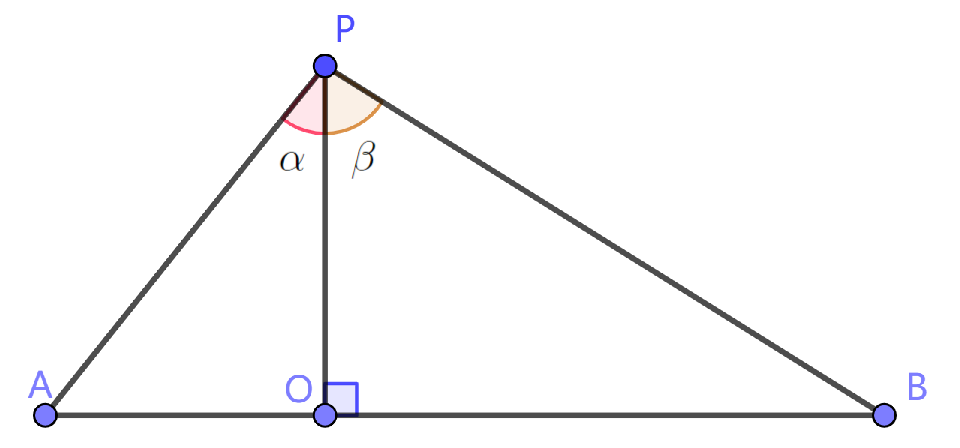
\includegraphics[width=0.5\textwidth]{和角正弦公式1.png}
    % \caption*{\texttt{垂心和外接圆}}
\end{figure}

让我们从两个锐角的和出发。如上图,$\alpha = \angle APO$和$\beta = \angle OPB$都是锐角,
$OP \perp AB$。$\triangle AOB$的面积是$\triangle AOP$、$\triangle BOP$面积之和。用相应的面积公式表示:
$$ \frac12 |AP||BP|\sin(\alpha + \beta) = \frac12 |AP||OP|\sin\alpha + \frac12 |OP||BP|\sin\beta$$
因此:
$$ \sin(\alpha + \beta) = \frac{|OP|}{|BP|}\sin\alpha + \frac{|OP|}{|AP|}\sin\beta$$
$\triangle AOP$、$\triangle BOP$都是直角三角形,所以$|OP| = |AP|\cos \alpha = |BP|\cos \beta$。
代入上式,就得到:
$$ \forall \,\, 0 < \alpha, \beta < 90^\circ , \,\,\, \sin(\alpha + \beta) = \sin\alpha \cos \beta + \cos \alpha \sin\beta.$$
这就是两锐角之和正弦值的公式,简称\textbf{和角正弦公式}。可以验证,当$\alpha$、$\beta$是零角或直角的时候,
公式仍然成立。所以,可以把公式的适用范围扩大为$0 \leqslant \alpha , \beta \leqslant 90^\circ$。

\begin{wrapfigure}[7]{r}{0.25\textwidth} %this figure will be at the right
    \vspace{-45pt}
    \flushright
    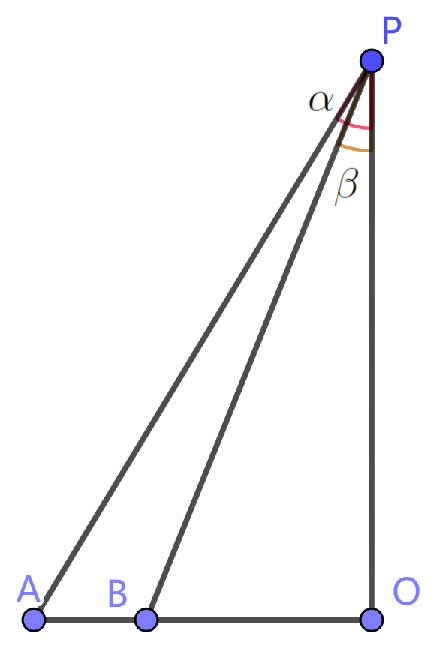
\includegraphics[width=0.24\textwidth]{差角正弦公式1.png}
\end{wrapfigure}

对于两锐角之差,可以用类似的方式推导。如右图,设$\alpha = \angle APO > \beta = \angle BPO$,
$\triangle AOP$的面积是$\triangle APB$、$\triangle OPB$面积之和。比照和角正弦公式的推导,可以得到:
$$ \forall \,\, 0 <  \beta < \alpha < 90^\circ , \,\,\, \sin(\alpha - \beta) = \sin\alpha \cos \beta - \cos \alpha \sin\beta.$$

是为两锐角之差正弦值的公式,简称\textbf{差角正弦公式}。可以验证,无论是当$\alpha$、$\beta$是零角或直角的时候,
还是$\alpha = \beta$的时候,公式仍然成立。
所以,可以把公式的适用范围扩大为$0 \leqslant \beta \leqslant \alpha \leqslant 90^\circ$。

注意到和角、差角正弦公式中都出现了角的余弦,我们可以据此推出和角、差角的余弦公式。
首先,假设$\alpha$、$\beta$、$\alpha - \beta$都是锐角。从和角正弦公式出发,可以得到这样的关系:
$$ \sin(\alpha) = \sin(\alpha - \beta + \beta) = \sin (\alpha - \beta) \cos \beta + \cos(\alpha - \beta) \sin\beta.$$
这个等式中只有$\cos(\alpha - \beta)$是未知的。根据差角正弦公式,可以得到:
\begin{align}
    \sin(\alpha) &= \sin (\alpha - \beta) \cos \beta + \cos(\alpha - \beta) \sin\beta \notag \\
    &= (\sin\alpha \cos \beta - \cos \alpha \sin\beta) \cos \beta + \cos(\alpha - \beta) \sin\beta \notag \\
    &= \sin\alpha \cos^2 \beta - \cos \alpha \sin\beta \cos \beta + \cos(\alpha - \beta) \sin\beta \notag
 \end{align}
因此
\begin{align}
    \sin\beta \cos(\alpha - \beta) &= \sin \alpha - \sin\alpha \cos^2 \beta + \cos \alpha \sin\beta \cos \beta \notag \\
    &= \sin \alpha (1 - \cos^2 \beta) + \cos \alpha \sin\beta \cos \beta \notag \\
    &= \sin\alpha \sin^2 \beta + \cos \alpha \sin\beta \cos \beta \notag \\
    &= \sin\beta (\sin\alpha \sin \beta +  \cos \alpha \cos \beta) \notag
 \end{align}
两边约去$\sin \beta$,就得到:
$$ \forall \,\, 0 <  \beta < \alpha < 90^\circ , \,\,\, \cos(\alpha - \beta) = \sin\alpha \sin \beta +  \cos \alpha \cos \beta. $$
这就是两锐角之差余弦值的公式,简称\textbf{差角余弦公式}。

同理,假设$\alpha$、$\beta$、$\alpha + \beta$都是锐角,从差角正弦公式出发,可以得到:
\begin{align}
      \sin(\alpha) &= \sin(\alpha + \beta - \beta) = \sin (\alpha + \beta) \cos \beta - \cos(\alpha + \beta) \sin\beta \notag \\
      &= (\sin\alpha \cos \beta + \cos \alpha \sin\beta) \cos \beta - \cos(\alpha + \beta) \sin\beta \notag \\
      &= \sin\alpha \cos^2 \beta + \cos \alpha \sin\beta \cos \beta - \cos(\alpha + \beta) \sin\beta \notag 
 \end{align}
因此
\begin{align}
    \sin\beta \cos(\alpha + \beta)  &= -\sin \alpha + \sin\alpha \cos^2 \beta + \cos \alpha \sin\beta \cos \beta \notag \\
    &= -\sin \alpha (1 - \cos^2 \beta) + \cos \alpha \sin\beta \cos \beta \notag \\
    &= -\sin\alpha \sin^2 \beta + \cos \alpha \sin\beta \cos \beta \notag \\
    &= \sin\beta (\cos \alpha \cos \beta - \sin\alpha \sin \beta) \notag
 \end{align}
两边约去$\sin \beta$,就得到:
$$  \cos(\alpha + \beta) = \cos \alpha \cos \beta - \sin\alpha \sin \beta. $$
这就是两锐角之和余弦值的公式,简称\textbf{和角余弦公式}。

要注意的是,上面的推导中,我们假设$\alpha$、$\beta$、$\alpha + \beta$是锐角。
然而,推导中涉及的项,除了$\cos(\alpha + \beta)$,都不要求$\alpha + \beta$是锐角。
另一方面,在和角余弦公式中,只要确定了$\alpha$、$\beta$,
就能计算$\cos \alpha \cos \beta - \sin\alpha \sin \beta$。
所以,$\alpha + \beta$是直角或钝角时,我们可以定义$\cos(\alpha + \beta)$为关于$x$的方程:
$$  x = \cos \alpha \cos \beta - \sin\alpha \sin \beta $$
的唯一解。这样,我们就定义了钝角的余弦值。当然,这样定义钝角余弦值,不好理解。
为了好理解,我们仿照正弦,给出互为补角的两角余弦的关系。这样,通过单个锐角的余弦值,就能得到钝角的余弦值了。

在和角余弦公式中,令较大角为直角,代入得到
$$  \forall \,\, 0 \leqslant \beta \leqslant 90^\circ , \,\,\, \cos(90^\circ + \beta) = - \sin\beta. $$

对锐角$\beta$来说,$90^\circ - \beta$也是锐角,于是:
$$ -\cos \beta = - \sin(90^\circ - \beta) = \cos(180^\circ - \beta). $$
这说明$ \cos(180^\circ - \beta) =  -\cos \beta$。\textbf{互为补角的两角,余弦值互为相反数}。

上一节中,我们让钝角的余弦等于其补角的相反数。现在我们看到,这个选择是合理的。
至此,我们可以写出余弦定理的统一形式:

\begin{tm}{\textbf{余弦定理}}\label{tm:2-4-10}
    设三角形$ABC$的内角$A,B,C$对边长度分别为$a,b,c$,则
    $$ a^2 = b^2 + c^2 - 2bc\cos A, \,\,\, b^2 = c^2 + a^2 - 2ca\cos B, \,\,\, c^2 = a^2 + b^2 - 2ab\cos C. $$
\end{tm}
余弦定理说明,三角形内角的余弦值,决定了它对边边长的平方与另两边边长的平方和的大小关系。
锐角的余弦值大于$0$,它对边边长的平方小于另两边边长的平方和。钝角的余弦值小于$0$,
它对边边长的平方大于另两边边长的平方和。直角的余弦值是$0$,它对边边长的平方等于另两边边长的平方和。

回到例题\ref{ex:2-2-10}第二题。之前我们算出$\cos C = -\frac{1}{15}$,说明$C$是钝角。
于是$\sin C = \sqrt{1 - \cos^2 C} \approx 0.9978$,
查表知锐角$180^\circ - C \approx 86.2^\circ$,即$\angle C \approx 93.8^\circ$。
同理,可以算得$\angle A \approx 29.9^\circ$,$\angle B \approx 56.3^\circ$。

我们用和角余弦公式定义了钝角的余弦。用同样的思路,我们考虑差角正弦公式:
$$ \sin(\alpha - \beta) = \sin\alpha \cos \beta - \cos \alpha \sin\beta $$
上式对$0 \leqslant \beta \leqslant \alpha \leqslant 90^\circ$成立。现在我们把它扩展到$\alpha < \beta$的情况。
也就是说,对小于零角的角度$\alpha - \beta$,我们定义$\sin (\alpha - \beta)$是关于$x$的方程:
$$ x = \sin\alpha \cos \beta - \cos \alpha \sin\beta $$
的唯一解。令$\alpha = 0$,就得到:
$$ \forall 0 \leqslant \beta \leqslant 90^\circ , \,\,\, \sin(- \beta) = -\sin\beta. $$
我们再把这个关系扩展到钝角。这样,我们就定义了负平角到正平角之间所有角度的正弦值。

最后,考虑差角余弦公式:
$$ \cos(\alpha - \beta) = \sin\alpha \sin \beta +  \cos \alpha \cos \beta. $$
比照差角正弦公式,对小于零角的角度$\alpha - \beta$,我们同样可以定义$\sin (\alpha - \beta)$是关于$x$的方程:
$$ x = \sin\alpha \sin \beta +  \cos \alpha \cos \beta $$
的唯一解。令$\alpha = 0$,就得到:
$$ \forall 0 \leqslant \beta \leqslant 90^\circ , \,\,\, \cos(- \beta) = \cos \beta. $$
同样把这个关系扩展到钝角,我们就定义了负平角到正平角之间所有角度的余弦值。

注意到负平角到正平角经历了整个周角,因此,定义了负平角到正平角的正弦和余弦值,
实际上就定义了所有角度的正弦和余弦值。至此,我们可以从锐角出发,
得到所有角度的正弦、余弦,而且它们的关系与和差角公式相容。

\begin{ex}
    \mbox{} \\
    \indent 1. 求$500^\circ$的正弦、余弦值。\\
    \indent 2. 求$-465^\circ$的正弦、余弦值。
\end{ex}
\begin{so}
    \mbox{} \\
    \indent 1. 首先加减周角,让角度落在负平角和正平角之间:
    $$\sin 500^\circ = \sin 140^\circ, \quad \cos 500^\circ = \cos 140^\circ.$$
    $140^\circ$是正钝角,因此取补角得到锐角:
    $$\sin 140^\circ = \sin 40^\circ, \quad \cos 140^\circ = -\cos 40^\circ.$$
    查表得到$\sin 500^\circ = \sin 40^\circ \approx 0.6428$,$\cos 500^\circ = -\cos 40^\circ \approx -0.766$。\\
    \indent 2. 首先加减周角,让角度落在负平角和正平角之间:
    $$\sin -465^\circ = \sin -105^\circ, \quad \cos -465^\circ = \cos -165^\circ.$$
    $140^\circ$是负钝角,取相反数变为正角,再取补角得到锐角:
    \begin{align}
        \sin -105^\circ = -\sin 105^\circ = -\sin 75^\circ, \notag \\
        \cos -105^\circ = \cos 105^\circ = -\cos 75^\circ. \notag 
    \end{align}
    查表得到$\sin -465^\circ = -\sin 75^\circ \approx -0.9659$,$\cos -465^\circ = -\cos 75^\circ \approx -0.2588$。
\end{so}

综上所述,可以这样总结任意角的正余弦与锐角正余弦的关系:
\begin{center}
    \fbox{
        \shortstack[l]{
            求任意角的正弦:\\
            1. 不断加减周角,直到角度落在$(-180^\circ, 180^\circ]$中。\\
            2. 如果是负角,取相反数变正角,结果取相反数。\\
            3. 如果是钝角,取补角变锐角,结果不变。\\
            求任意角的余弦:\\
            1. 不断加减周角,直到角度落在$(-180^\circ, 180^\circ]$中。\\
            2. 如果是负角,取相反数变正角,结果不变。\\
            3. 如果是钝角,取补角变锐角,结果取相反数。
        }
    }
\end{center}

\begin{xt}\label{xt:2-4-10}
    \mbox{} \\
    \indent 1. 验证:和角、差角公式对负平角到正平角中的角度成立。 \\
    \indent 2. 证明正弦和余弦的\textbf{倍角公式}:
    \begin{align}
        \forall \,\, 0 \leqslant \alpha \leqslant 90^\circ , \,\,\, & \sin 2\alpha = 2\sin \alpha \cos \alpha \notag \\
        & \cos 2\alpha = 2\cos^2 \alpha - 1 \notag 
    \end{align}
    \indent 3. 证明正弦和余弦的\textbf{半角公式}:
    \begin{align}
        \forall \,\, 0 \leqslant \alpha \leqslant 180^\circ , \,\,\, & \sin \frac{\alpha}{2} = \sqrt{\frac{1 - \cos \alpha}{2}}  \notag \\
        & \cos \frac{\alpha}{2} = \sqrt{\frac{1 + \cos \alpha}{2}} \notag
    \end{align}
    \indent 4. 证明正弦和余弦的\textbf{积化和差公式}:
    \begin{align}
        \cos \alpha \cos \beta &= \frac12 (\cos (\alpha + \beta) + \cos (\alpha - \beta)) \notag \\
        \sin \alpha \sin \beta &= \frac12 (\cos (\alpha - \beta) - \cos (\alpha + \beta)) \notag \\
        \sin \alpha \cos \beta &= \frac12 (\sin (\alpha + \beta) + \sin (\alpha - \beta)) \notag 
    \end{align}
    \indent 5. 证明正弦和余弦的\textbf{和差化积公式}:
    \begin{align}
        \sin \alpha \pm \sin \beta &= 2\sin \frac{\alpha \pm \beta}{2} \cos \frac{\alpha \mp \beta}{2} \notag \\
        \cos \alpha + \cos \beta &= 2\cos \frac{\alpha + \beta}{2} \cos \frac{\alpha - \beta}{2} \notag \\
        \cos \alpha - \cos \beta &= -2\sin \frac{\alpha + \beta}{2} \sin \frac{\alpha - \beta}{2} \notag 
    \end{align}
    \indent 5. 设平行四边形$ABCD$的相邻两边长为$a,b$,两对角线长为$u,v$,证明:$u^2 + v^2 = 2a^2 + 2b^2$。 \\
    \indent 6. 设$\triangle ABC$三边长分别为$a,b,c$,证明:
    $$\sin A = \frac{\sqrt{(b+c-a)(a-b+c)(a+b-c)(a+b+c)}}{2bc}.$$ 
    \indent 7. 设$\triangle ABC$周长的一半为$p$,证明:$S_{\triangle ABC} = \sqrt{p(p-a)(p-b)(p-c)}$。 \\
    \indent 8. $\triangle ABC$一边的长度是另一边的$2$倍。设$A$是$\triangle ABC$最大的内角,证明:$\cos A \leqslant 0.25$。

\end{xt}

\section{正切函数和余切函数}

历史上,除了正弦函数和余弦函数,数学家们还发明了别的函数来讨论角度。\textbf{正切函数}和\textbf{余切函数}就是两种常用的函数。

如下图,单位圆的切线$l$与锐角$\angle AOP$的终边交于$Q$,定义$\angle AOP$的\textbf{正切}(\textbf{值})为
$\tan\angle AOP = |AQ|$,\textbf{余切}(\textbf{值})为$\cot\angle AOP = \frac{1}{|AQ|}$。
也就是说,我们用角截切线的长度来度量角的大小。按照定义,\textbf{同角的正切值和余切值互为倒数}。

\begin{wrapfigure}[7]{r}{0.25\textwidth} %this figure will be at the right
    \vspace{-15pt}
    \flushright
    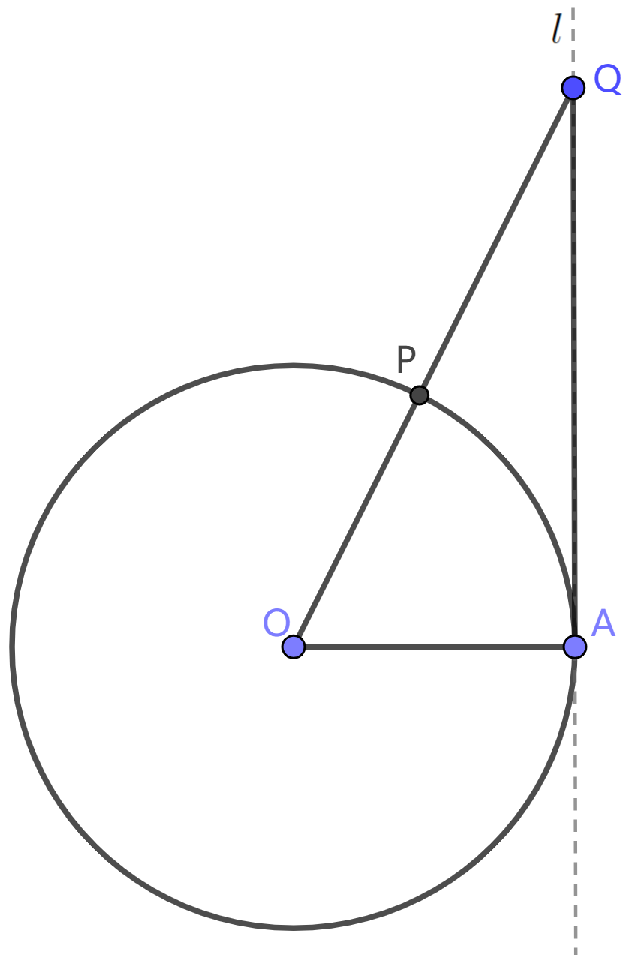
\includegraphics[width=0.24\textwidth]{正切函数1.png}
\end{wrapfigure}

和正弦、余弦一样,我们可以定义正切、余切函数。
要注意的是,正切函数对零角和锐角有定义,但对直角没有定义。余切函数对锐角和直角有定义,对零角没有定义。

不难证明:
$$ \forall \,\, 0 < \alpha < 90^\circ, \,\,\, \tan \alpha = \frac{\sin \alpha}{\cos \alpha}, \,\,\, \cot \alpha = \frac{\cos \alpha}{\sin \alpha}$$
换句话说,可以用锐角的正弦和余弦定义它的正切和余切。不难推出:
$$ \forall \,\, 0 < \alpha < 90^\circ, \,\,\, \tan (90^\circ - \alpha) = \cot \alpha, \,\,\, \cot (90^\circ - \alpha) = \tan \alpha. $$
零角的正切是$0$,直角的余切是$0$。
从零角开始,随着角度增大,正切值不断增大。从直角开始随着角度减小,余切值不断减小。
$\cos 45^\circ = \sin (90^\circ - 45^\circ) = \sin 45^\circ $,
因此$\tan 45^\circ = \cot 45^\circ = 1$。

反过来,也可以用锐角的正切和余切定义它的正弦和余弦:
$$ \forall \,\, 0 < \alpha < 90^\circ, \,\,\, \sin \alpha = \sqrt{\frac{1}{1 + \cot^2 \alpha}}, \,\,\, \cos \alpha = \sqrt{\frac{1}{1 + \tan^2 \alpha}}$$

对其他角度,我们保持正切、余切和正弦、余弦的关系,定义
$$ \forall \,\,  \alpha, \,\,\, \tan \alpha = \frac{\sin \alpha}{\cos \alpha}, \,\,\, \cot \alpha = \frac{\cos \alpha}{\sin \alpha}$$
这样,除去分母为零的情况,我们定义了任意角的正切和余切。

从正弦和余弦的和差角公式,可以推出正切和余切的和差角公式:
\begin{align}
    \forall 0 \leqslant \alpha, \beta < 90^\circ, & \notag \\
    \tan (\alpha + \beta) &= \frac{\sin (\alpha + \beta)}{\cos (\alpha + \beta)} = \frac{\sin\alpha \cos \beta + \cos \alpha \sin\beta}{\cos \alpha \cos \beta - \sin\alpha \sin \beta} \notag \\
    &= \frac{\tan \alpha + \tan \beta}{1 - \tan \alpha \tan \beta} \notag   \\ 
    \tan (\alpha - \beta) &= \frac{\sin (\alpha - \beta)}{\cos (\alpha - \beta)} = \frac{\sin\alpha \cos \beta - \cos \alpha \sin\beta}{\cos \alpha \cos \beta + \sin\alpha \sin \beta} \notag \\
    &= \frac{\tan \alpha - \tan \beta}{1 + \tan \alpha \tan \beta} \notag 
\end{align}
\begin{align}
    \forall 0 < \alpha, \beta \leqslant 90^\circ, & \notag \\
    \cot (\alpha + \beta) &= \frac{\cos (\alpha + \beta)}{\sin (\alpha + \beta)} = \frac{\cos \alpha \cos \beta - \sin\alpha \sin \beta}{\sin\alpha \cos \beta + \cos \alpha \sin\beta} \notag \\
    &= \frac{\cot \alpha \cot \beta - 1}{\cot \alpha + \cot \beta} \notag  \\
    \cot (\alpha - \beta) &= \frac{\cos (\alpha - \beta)}{\sin (\alpha - \beta)} = \frac{\cos \alpha \cos \beta + \sin\alpha \sin \beta}{\sin\alpha \cos \beta - \cos \alpha \sin\beta} \notag \\
    &= \frac{\cot \alpha \cot \beta + 1}{\cot \alpha - \cot \beta}  \notag 
\end{align}
以上关系可以简写为:
\begin{align}
    \tan (\alpha \pm \beta) &= \frac{\tan \alpha \pm \tan \beta}{1 \mp \tan \alpha \tan \beta} \notag \\
    \cot (\alpha \pm \beta) &= \frac{\cot \alpha \cot \beta \mp 1}{\cot \alpha \pm \cot \beta} \notag
\end{align}
除去分母为零的情况,任意角的正切和余切也满足以上的和差角公式。

三角形中,内角之和为平角。因此,两角之和的正切值是第三个角正切值的相反数:
\begin{align}
    \tan C &= \tan (180^\circ - (A + B)) = - \tan (A + B) \notag \\
    &= - \frac{\tan A + \tan B}{1 - \tan A \tan B}. \notag 
\end{align}
于是:
\begin{align}
    \tan C (1 - \tan A \tan B) &= - \tan A - \tan B, \notag \\
    \tan A + \tan B + \tan C &= \tan A \tan B \tan C. \notag
\end{align}
\begin{tm}{\textbf{正切定理}}\label{tm:2-5-10}
    三角形内角的正切值之和等于它们的乘积。
\end{tm}
正切定理和正弦定理、余弦定理不同。它并不涉及三角形的边,是纯粹关于角的定理。
使用正切定理无法解决边角关系的问题,但可以比较方便地给出三角形内角的关系。
利用正切和余切的倒数关系,可以写出关于余切的类似结论:
\begin{tm}{\textbf{余切定理}}\label{tm:2-5-20}
    三角形$ABC$内角的余切值满足:
    $$ \cot A \cot B + \cot B \cot C + \cot C \cot A = 1.$$
\end{tm}

\begin{xt}\label{xt:2-5-10}
    \mbox{} \\
    \indent 1. 证明正切和余切的\textbf{倍角公式}:
    \begin{align}
        \forall \,\, 0 < \alpha < 45^\circ, \,\,\,& \tan 2\alpha = \frac{2\tan \alpha}{1 - \tan^2 \alpha} & \notag \\
        &\cot 2\alpha = \frac{\cot^2 \alpha - 1}{2 \cot \alpha} & \notag 
    \end{align}
    \indent 2. 证明正切和余切的\textbf{半角公式}:
    \begin{align}
        \forall \,\, 0 < \alpha < 180^\circ, \,\,\,& \tan \frac{\alpha}{2} = \frac{\sin \alpha}{1 + \cos \alpha} = \frac{1 - \cos \alpha}{\sin \alpha} = \sqrt{\frac{1 - \cos \alpha}{1 + \cos \alpha}}\notag \\
        & \cot \frac{\alpha}{2} = \frac{1 + \cos \alpha}{\sin \alpha} = \frac{\sin \alpha}{1 - \cos \alpha} = \sqrt{\frac{1 + \cos \alpha}{1 - \cos \alpha}} \notag 
    \end{align}
    定义锐角$\alpha$的\textbf{正割值}($\sec \alpha$)和\textbf{余割值}($\csc \alpha$):
    \begin{align}
        \sec \alpha &= \frac{1}{\cos \alpha}, \,\,\, \csc \alpha = \frac{1}{\sin \alpha}. \notag 
    \end{align}
    \indent 3. 证明:锐角的正割等于它的余角的余割,锐角的余割等于它的余角的正割。\\
    \indent 4. 证明:$ 1 + \tan^2 \alpha = \sec^2 \alpha , \,\,\, 1 + \cot^2 \alpha = \csc^2 \alpha. $\\
    \indent 5. 证明\textbf{万能公式}:
    \begin{align}
        \forall 0 < \alpha < 180^\circ, & \mbox{ 记} \tan\frac{\alpha}{2} = t, \,\,\, \mbox{则:}\notag \\
        \sin \alpha = \frac{2t}{1 + t^2}, & \,\,\,\,\, \tan \alpha = \frac{2t}{1 - t^2}, \,\,\,\,\,\, \sec \alpha = \frac{1 + t^2}{1 -t^2}, \notag \\
        \cos \alpha = \frac{1 -t^2}{1 + t^2}, & \,\,\,\,\,\, \cot \alpha = \frac{1 - t^2}{2t}, \,\,\,\,\,\, \csc \alpha = \frac{1 + t^2}{2t}. \notag  
    \end{align}
\end{xt}

\section{多边形的边角关系}

多边形的边和角没有直接对应关系。因此,多边形的边角关系,要通过对角线来间接建立。
比如,圆内接凸四边形$ABCD$中,对角之和为平角。根据余弦定理,
\begin{align}
    |AC|^2 &= |AB|^2 + |BC|^2 -2|AB||BC|\cos\angle ABC \notag \\
    &= |AD|^2 + |DC|^2 -2|AD||DC|\cos\angle CDA \notag
\end{align}
于是,我们得到圆内接凸四边形的内角和四边边长的关系:
\begin{align}
    \cos\angle ABC = -\cos \angle CDA &= \frac{|AB|^2 + |BC|^2 - |CD|^2 - |DA|^2 }{2(|AB||BC| + |CD||DA|)}, \notag \\
    \cos\angle BCD = -\cos \angle DAB &= \frac{|BC|^2 + |CD|^2 - |DA|^2 - |AB|^2 }{2(|BC||CD| + |DA||AB|)}. \notag 
\end{align}

另一个例子是正多边形。设单位圆$O$的内接正$n$边形边长为$b_n$,
连接圆心$O$和相邻两顶点$A,B$,$\triangle OAB$是等腰三角形。
正$n$边形内角为$\alpha_n = \frac{(n-2)180^\circ}{n}$,
因此$\angle OAB = -\angle OBA = \frac{\alpha_n}{2} = \frac{(n-2)90^\circ}{n}$,
$\angle AOB = \frac{360^\circ}{n}$。根据正弦定理,
$$ \frac{b_n}{\sin \angle AOB} = \frac{1}{\sin \angle OAB}.$$
因此
$$b_n = \frac{\sin \frac{360^\circ}{n}}{\sin \frac{(n-2)90^\circ}{n}} = \frac{\sin \frac{360^\circ}{n}}{\cos \frac{180^\circ}{n}}.$$

为了方便,记$\beta_n = \frac{180^\circ}{n}$,则$b_n = \frac{\sin 2\beta_n}{\cos \beta_n} = 2\sin \beta_n$。
于是,正$n$边形的周长是$nb_n = 2n\sin \beta_n$。

\begin{xt}\label{xt:2-6-10}
    \mbox{} \\
    \indent 1. 求单位圆内接正$12$边形的周长。\\
    设圆内接四边形$ABCD$面积为$S$,周长为$2p$,\\
    \indent 2. 证明$S = \frac12 \sin \angle ABC (|AB||BC| + |CD||DA|)$。 \\
    \indent 3. 证明$S^2 = (p - |AB|)(p - |BC|)(p - |CD|)(p - |DA|)$。\\
    \indent 4. 对一般的四边形$ABCD$,如何用$|AB|, |BC|, |CD|, |DA|$和$\frac{\angle ABC + \angle CDA}{2}$表示它的面积$S$?
\end{xt}

\chapter{从或许到确定}
预测未来,是人类社会的重要活动。合理有效地预测未来,是社会文明进步的标志。
中华文明作为农耕文明,很早就懂得预测未来的重要性。
历法、史书、节气,都是我们的祖先为了后人更好地预测未来,留下的经验总结。

生产活动中,预测尤其重要。比如,农牧业、渔业、运输业等行业需要预测天气,
销售行业需要预测产品的市场需求。科学研究和工程制造中,如果能够提前知道产品在各种各样的情境和场景下的性能,
可以节约大量人力物力。社会要发展,就需要更高的预测水平。

\section{事件和见知}

如何判断某件事情将来会不会发生?我们要依赖已有的知识和经验。日常生活中,
我们会说“明天大概要下雨”、“今年冬天肯定很冷”、“我明天大概去不了了”。根据已有条件,
有些事情必然发生,有些事情或许会发生,有些事情不可能发生。事情发生与否,取决于某些条件。
我们把这样的事情叫作\textbf{随机事件},简称\textbf{事件}。
在已知条件下,如果某事件必然发生,就说它是\textbf{必然事件};
如果某事件必然不发生,就说它是\textbf{不可能事件};
如果某事件或许会发生,就说它是\textbf{或然事件}。数学中,研究这些事情的理论叫作概率论。

概率论假定,我们关心的随机事件有某些恒定的内在规律,受某些固有未知因素的影响。
概率论通过研究这些内在规律和因素,预测事件是否会发生。

如何描述一个事件?从客观的角度,我们可以把“发生一件事”看成事物状态、形势局面的改变。
一件事是否发生,可以用改变后的状态或局面表示。我们也许无法确定未来事物发展成哪个状态、形势走向哪个局面,
但我们可以事先确定事物未来所有可能的状态、所有可能出现的局面。

比如,我们无法确定明天杭州是否下雨,但我们知道,在明天杭州是否下雨这个问题上,只可能出现两个结局:下雨或不下雨。
又比如,我们投一个骰子前,无法确定朝上一面的点数,但我们知道,投出的骰子最终只有六个状态:
朝上一面是$1,2,3,4,5$或$6$点。这些最终状态、局面是\textbf{互斥}的。比如明天杭州不可能既下雨又不下雨,
骰子停下之后不可能既是$1$点朝上又是$2$点朝上。

我们把所有可能的最终状态或局面看成一个集合,集合中的每个元素称为事情的\textbf{终态}或\textbf{结局}。
比如,考虑明天杭州是否下雨这个问题时,所有结局构成$\{\mbox{下雨}, \mbox{不下雨}\}$这个集合,
每次投骰子时,骰子的终态构成$\{1,2,3,4,5,6\}$这个集合。我们把这个集合叫作\textbf{终集},即终态的全集。
我们可以把相关的事件用终集的子集表示。比如,“明天杭州下雨”对应$\{\mbox{下雨}\}$这个子集,
“骰子点数是偶数”对应$\{2,4,6\}$这个子集。事物发展的终态如果在子集里,就说明事件发生了,否则事件没有发生。

单元集也对应着事件。我们把这些事件叫做\textbf{基本事件}。
不是任何其他事件的交集的事件,叫做基本事件。比如$\{1\}$对应的“骰子点数是$1$”就是基本事件。
基本事件是各种事件的“基本单元”,它们通过合并形成别的事件。基本事件之间是互斥事件,它们是终集的分划。

终集可以是有限的,也可以是无限的。目前我们只讨论有限的情况。
要注意的是,随着问题的条件、环境、思考问题的角度发生变化,终集也会变化。
比如,我们考虑明天杭州下雨的问题时,可能要把准备经过杭州的台风“凤凰”也考虑在内。
台风“凤凰”也许继续靠近,也许转向。这时,我们的终集是:
$$\{\mbox{台风靠近且下雨}, \mbox{台风靠近且不下雨}, \mbox{台风转向且下雨}, \mbox{台风转向且不下雨}\}$$

而“明天杭州下雨”对应子集$\{\mbox{台风靠近且下雨}, \mbox{台风转向且下雨}\}$。

对于随机事件,如果我们知道得更多,就能作出更准确的预测。
比如,如果我们不知道台风的情况,那么即便我们把终集依照“台风是否继续靠近”划分,
我们能把握的也只是$\{\mbox{台风靠近且下雨}, \mbox{台风转向且下雨}\}$、
$\{\mbox{台风靠近且不下雨}, \mbox{台风转向且不下雨}\}$两个事件,
与$\{\mbox{下雨}\}, \{\mbox{不下雨}\}$并没有不同。
如果我们掌握了台风的动向,我们就希望把$\{\mbox{下雨}\}$分成\\   
$\{\mbox{台风靠近且下雨}\}$和$\{\mbox{台风转向且下雨}\}$来讨论了。
可以说,随着我们对事物、形势的认知增加,我们的终集会越来越“细”。

为了描述认知增加的过程,我们从最“细”的终集出发,定义每个阶段的\textbf{知集},代替不同阶段的终集。
知集是最“细”终集的子集构成的集合,满足:

\begin{enumerate}
    \item 空集属于知集;
    \item 如果集合$A$属于知集,那么$A$的补集也属于知集;
    \item 如果集合$A$和$B$属于知集,那么它们的并集也属于知集。
\end{enumerate}

知集表示我们每个阶段的认知。我们根据当前的认知来讨论各种事件。
比如,在杭州下雨的例子里,可以有两个知集,分别是:
$$ S_1 = \big\{\varnothing, \{\mbox{AR}, \mbox{DR}\},\{\mbox{AN}, \mbox{DN}\}, \{\mbox{AR}, \mbox{AN}, \mbox{DR}, \mbox{DN}\} \big\}$$

和
\begin{align}
    S_2 &= \big\{ \varnothing, \{\mbox{AR}\}, \{\mbox{AN}\}, \{\mbox{DR}\}, \{\mbox{DN}\}, \{\mbox{AR}, \mbox{AN}\}, \{\mbox{AR}, \mbox{DR}\}, \{\mbox{AR}, \mbox{DN}\}, \notag \\
    & \{\mbox{AN}, \mbox{DR}\}, \{\mbox{DN}, \mbox{AN}\}, \{\mbox{DR}, \mbox{DN}\},  \{\mbox{AR}, \mbox{AN}, \mbox{DR}\}, \{\mbox{AR}, \mbox{AN}, \mbox{DN}\}, \notag \\
    &  \{\mbox{AR}, \mbox{DR}, \mbox{DN}\},  \{\mbox{AN}, \mbox{DR}, \mbox{DN}\}, \{\mbox{AR}, \mbox{AN}, \mbox{DR}, \mbox{DN}\} \big\} \notag 
\end{align}
其中$\mbox{AR}, \mbox{AN}, \mbox{DR}, \mbox{DN}$分别表示
“台风靠近且下雨”、“台风靠近且不下雨”、“台风转向且下雨”和”台风转向且不下雨“。
可以看出,$S_1$是$S_2$的子集。$S_1$到$S_2$的过程,就是对台风认知加深的过程。

这种描述下,不同的知集就对应不同“粗细”的终集。每个知集都对应自己的基本事件。
这时候的基本事件不一定是单元集。比如,$\{\mbox{AR}, \mbox{DR}\}$在$S_1$中是基本事件,在$S_2$中就不是基本事件了。

\begin{xt}
    写出以下问题的终集和知集。\\
    \indent 1. 我国朱鹮从东北省份向南迁徙的路线有三条:西线、中线和东北线。
    小明想知道黑龙江省的某只朱鹮沿哪条路线南迁。\\
    \indent 2. 某航空公司规定:作为补偿,飞机晚点一小时以上,返还全票票价的$40\%$;
    如果晚点三小时以上,返还全票票价的$75\%$。乘客实际购票价低于前述返还价格的,
    返还乘客实际购票价。航班因晚点取消,且乘客自愿接受转乘下一班机的,公司协助补票,
    实施“就低返利”政策:按照下一班机实时票价和乘客最初购票价的较低者计算新票价,多则退还差价;
    并另外补偿新票价的$30\%$。某乘客购票后,在候机时被告知飞机可能晚点,他试着分析可能得到的晚点补偿。
\end{xt}

\section{概率和分布}

预测随机事件时,我们除了关心会发生什么事情,还关心事情有多大可能发生。
当我们说“这事百分之百能成”,“他八成还在路上”,“他的话只有三分准头”,
我们认为某些事情比另一些事情更可能发生。习惯上,我们用数来描述事情有多大可能发生。
在数学中,我们把这个做法称为\textbf{事件的概率}。

我们用不大于$1$的非负实数表示事件的概率。约定不可能事件的概率是$0$,必然事件的概率是$1$。
事件的概率越大,越有可能发生。
此外,事件的概率应当和事件之间的关系相符。两个互斥事件同时发生的概率应该是$0$,
至少有一个发生的概率应该是它俩概率的和。用集合的语言来说,空集的概率应该是$0$,
终集的概率应该是$1$;两个集合不相交,那么它们的并集的概率等于它们概率的和。

我们习惯用映射$\mathbb{P}$来记录概率。把事件$A$的概率记为$\mathbb{P}(A)$。
比如,我们说明天八成会下雨,可以写成$\mathbb{P}(\{\mbox{下雨}\}) = 0.8$。
不至于混淆时,也可以省略表示集合的大括号,写成:$\mathbb{P}(\mbox{下雨}) = 0.8$。

基本事件两两互斥,并集是终集(全集)。所以,基本事件的概率之和等于$1$。

举例来说,投骰子的时候,我们一般认为投出$1,2,3,4,5,6$点的可能性都一样大,
即每个基本事件的概率都相等。于是它们各自的概率是六分之一。
据此,可以算出任何事件的概率。比如,“投出$5$点或以上”的概率是“投出$5$点”的概率加上“投出$6$点”的概率,
也就是三分之一。如果我们知道骰子有问题,比如投出$6$点的可能性是其他任一点数的$2$倍,
那么“投出$6$点”的概率是七分之二;投出其他点数,比如“投出$3$点”的概率是七分之一;
而“投出$5$点或以上”的概率是七分之三。

终集是有限集合的时候,对每个知集来说,只要知道了其中每个基本事件分配到的概率(称为\textbf{概率分布}),
就可以推出知集里其他事件的概率。

\begin{sk}
    同一个终集下的不同知集中,同一个事件的概率是否相同?
\end{sk}

\section{二项分布和均匀分布}

我们来看两种简单的概率分布。

考虑只有两个终态$a, b$的终集,两个基本事件$\{a\}, \{b\}$概率之和是$1$。
设其中一个的概率是$p$,则另一个的概率是$1-p$。我们把这样的概率分布叫作\textbf{二项分布}。
举例来说,如果我们认为明天杭州下雨的概率是$0.7$,不下雨的概率就是$1-0.7=0.3$。
我们说,我们认为明天杭州下雨的问题服从二项分布。

又比如:抛一枚硬币,我们认为正面朝上的概率是$0.52$,那么反面朝上的概率就是$1 - 0.52 = 0.48$。
我们说,我们认为抛这枚硬币的问题服从二项分布。
为了好说话,我们会在两个基本事件中选一个我们更关心的,称为\textbf{正面事件},把另一个称作\textbf{反面事件}。
如果正面事件的概率是$p$,就说问题服从系数为$p$的二项分布。

终集为$\{a, b\}$的二项分布,包括四个事件,分别对应$\varnothing, \{a\}, \{b\}, \{a, b\}$四个子集。
设$\{a\}$是正面事件,概率为$p$,那么这四个事件的概率分别是$0$、$p$、$1-p$和$1$。

对于元素更多的终集,情况更加复杂。我们考虑一种简单情形:每个基本事件的概率相等。
这样的概率分布称为\textbf{等概率分布}或\textbf{均匀分布}。
比如,投骰子时,如果我们认为每面朝上的概率都相等,就说投骰子服从均匀分布。

假设终集有$n$个终态,那么每个基本事件的概率就是$\frac{1}{n}$。
对于任意事件,我们可以数一下事件包含了几个终态,用终态个数除以所有终态的个数,
就是它的概率。我们把这个性质写作:
$$ \mathbb{P}(A) = \frac{|A|}{|S|} $$
其中$|A|$表示事件$A$作为集合的元素个数,$|S|$表示终集$S$的元素个数。 
比如,服从均匀分布的投骰子问题中,要求“大于$2$点”的概率,我们数一下事件$\{3,4,5,6\}$,
它包含了$4$个终态,所以“大于$2$点”的概率是$4 \times \frac{1}{6} = \frac{2}{3}$。

\begin{xt}
    \mbox{} \\
    \indent 1. 把$1$到$100$分别写在小纸条上放入黑箱里,随意抽取一张,
    抽到的数是素数的概率是多少?完全平方数的概率是多少?各位数字乘积大于$10$的概率是多少? \\
    \indent 2. 有没有以全体自然数为终集的均匀分布?为什么?说说你的理由。
\end{xt}

% \section{条件概率和独立事件}
% 讨论随机事件,总要知道前提条件。只有明确了前提条件,才能讨论事件的概率。
% 为了研究不同的前提条件对事件的影响,我们引入条件概率的概念。

% 仍以“明天杭州是否下雨”为例。我们讨论台风“凤凰”动向对下雨概率的影响,可以说:
% “如果台风靠近,那么下雨的概率有$90\%$”、“如果台风转向,那么不下雨的概率为$40\%$”。
% 这里我们把台风靠近与否作为明天杭州下雨的前提条件。以上两句话可以记作:
% $$ \mathbb{P} (\{\mbox{下雨}\} \, | \, \{\mbox{台风靠近}\}) = 0.9, \quad \mathbb{P} (\{\mbox{不下雨}\} \, | \, \{\mbox{台风转向}\}) = 0.4$$
% 从知集$S_2$的角度,$\mathbb{P} (\{\mbox{下雨}\} \, | \, \{\mbox{台风靠近}\}$应该记为:
% $$  \mathbb{P} (\{\mbox{台风靠近且下雨}, \mbox{台风转向且下雨}\} \, | \, \{\mbox{台风靠近}\}$$
% 但我们知道,在“台风靠近”的前提条件下,

\section{排列和组合}
均匀分布的问题里,事件的概率只和它包含的终态的个数以及所有终态的个数有关。因此,在相关的一些问题里,
我们关心如何计出事件包含的终态的个数。

\begin{ex}
    将编号为$1,2,3$的$3$个小球排成一列,最左边的球是$1$的概率是多少?
\end{ex}
要知道事件“最左边的球是$1$”的概率,用“最左边的球是$1$”包含的终态个数除以所有终态的个数。
怎么计算“最左边的球是$1$”包含的终态个数和所有终态的个数呢?

首先考虑所有终态的个数:将编号为$1,2,3$的$3$个小球排成一列,有多少种方法?

不妨设三个球从左到右排列。无论排列方式如何,三个球分别占据“左”、“中”、“右”三个位置。
从左边开始,把球一个个放到位置上。左边的位置可以放三个球中任何一个,因此有$3$种方法。
按任一种方法放好左边的球以后,中间的位置可以放剩余两个球中任何一个,因此有$2$种方法。
按任一种方法放好中间的球以后,右边的位置可以放最后一个球,只有$1$种方法。
于是一共有$3\times 2\times 1 = 6$种方法。

如果最左边的球是$1$,有多少种方法?这时左边的位置已经放好了$1$号球,因此中间的位置还有两种放法。
任一种方法放好中间的球以后,右边的位置放最后一个球,只有$1$中方法。因此,一共有$2\times 1 = 2$种方法。

综上所述,“最左边的球是$1$”的概率是:
$$ \mathbb{P}(\mbox{最左边的球是}1) = \frac{2}{6} = \frac{1}{3}. $$

我们把$n$个互不相同的物品排成一列的方法数目称为$n$\textbf{排列数},记作$P_n$。
比如,编号为$1,2,3$的$3$个小球排成一列的方法数目就叫做“$3$排列数”,记作$P_3$。

对于一般的自然数$n$,$n$排列数是$n-1$排列数的$n$倍。
这是因为,如果把$n$个互不相同的物品排成一列,第一个位置总可以放$n$个物品中的任何一个,
有$n$种方法。按任一种方法放好第一个位置后,剩下的$n-1$个位置摆放剩下的$n-1$个物品的方法数目,
恰好就是$n-1$排列数。

因此,用归纳法可以证明,$n$排列数就是$n$乘以$n-1$乘以$n-2$……直到乘以$1$的乘积。比如,
$5$排列数就是$5\times 4\times 3\times 2\times 1 = 120$。

如果我们把从$n$乘到$1$的计算看成关于$n$的函数的话,这个函数叫做($n$的)\textbf{阶乘},记作$n!$。
$n$排列数就是$n$的阶乘。

\begin{ex}
    将$3$个红球和$2$个白球组成一列,最左边的球是红球的概率是多少?
\end{ex}
我们仍然先计算$3$个红球和$2$个白球组成一列的方法数。
这里球只有红白两种颜色的分别。同色的球没有差别。如果我们把球编号,$1,2,3$号球是红球,$4,5$号球是白球,
那么,按照编号排列,有$5! = 120$种方法。不过,$1-2-3-4-5$和$2-3-1-4-5$其实是同一种方法。
因为$1,2,3$号球都是红球,并没有差别。把$1-2-3-4-5$里的$3$个红球任意改变次序,都不影响结果。同理,
把$1-2-3-4-5$里的$2$个白球任意改变次序,都不影响结果。$3$个红球的排列方法有$3! = 6$种,$2$个
白球的排列方法有$2! = 2$种,于是这$6\times 2 = 12$种方法都对应同一种结果。也就是说,带编号的$12$个排列方法
对应一种不带编号的排列方法。因此,实际上只有$\frac{5!}{3!2!} = 10$种排列方法。

我们把不带编号的排列方法称为\textbf{组合数}或\textbf{选列数}。
比如,$3$个红球和$2$个白球组成一列的方法数目叫做“$3,2$组合数”,或“$5$选$3$”
(因为也可以看作从$5$个位置里选$3$个放红球),记作$C_5^3$或$5 \choose 3$。

如果最左边的球是红球,那么剩下的$4$个位置要放$2$个红球、$2$个白球。于是,一共有$C_4^2$种方法。计算可知:
$$ C_4^2 = \frac{4!}{2!\times 2!} = \frac{24}{2\times 2} = 6.$$
即一共有$6$种方法。因此最左边的球是红球的概率是:
$$ \mathbb{P}(\mbox{最左边的球是红球}) = \frac{C_4^2}{C_5^3} = \frac{6}{10} = \frac{3}{5}.$$

一般来说,“$n$选$m$”也可以用阶乘计算:
$$ C_n^m = \frac{n!}{m!(n-m)!} $$

容易发现:“$n$选$m$”等于“$n$选$n-m$”。比如,$5$选$3$等于$5$选$2$。
用红球和白球的例子,可以理解为:$3$个红球和$2$个白球组成一列的方法数目,
等于$3$个白球和$2$个红球组成一列的方法数目。

掌握了排列数和组合数,我们就可以计算一些复杂问题里终态的个数。

\begin{xt}
    \mbox{} \\
    \indent 1. $5$个红球和$3$个白球排成一列,有多少种方法?\\
    \indent 2. $2$个红球、$3$个白球和$2$个黄球排成一列,有多少种方法?\\
    \indent 3. 从编号$1,2,3,4,5$的$5$个球中选出$3$个排成一列,有多少种方法?这个数目叫做$5,3$排列数。
    试求一般情况下$n,m$排列数(从编号为$1$到$n$的$n$个球中选出$m$个排成一列的方法数目)的公式。\\
    \indent 4. 设有两个正整数$m < n$,证明:$m!$整除$n!$。
\end{xt}

\chapter{三段论}

我们已经学习过换质法和换位法。它们都属于直接推理,即通过一个前提得出一个结论。
通过多个前提得出结论,称为\textbf{间接推理}。\textbf{三段论}是一种常见的间接推理。

\section{三段论的结构}
三段论是由三个判断构成的推理,一共涉及三个概念,
每个判断中的主语和断语分别涉及一个概念,
每个概念在两个判断中各出现一次。例如:
\begin{quotation}
    \noindent \ding{172}所有的科学规律都是不以人们的意志为转移的。\\
    \ding{173}物理学规律是科学规律。\\
    \ding{174}所以,物理学规律是不以人们的意志为转移的。
\end{quotation}
就是一个三段论。它包含两个前提(\ding{172}和\ding{173})和一个结论(\ding{174})共三个判断,
涉及三个概念:“科学规律”、“物理学规律”和“不以人们的意志为转移的”。
每个概念在两个判断中分别出现一次。比如“科学规律”就在\ding{172}和\ding{173}中各出现一次。

组成三段论的每个判断可以是简单判断,也可以是复合判断。
这里我们只研究由三个简单判断组成的三段论。

我们把三段论涉及的三个概念称为\textbf{大项}、\textbf{中项}和\textbf{小项}。大项是结论的断语中出现的概念,
中项是在两个前提中分别出现的概念,小项是结论的主语中出现的概念。以上的例子中,
“不以人们的意志为转移的”是大项,“科学规律”是中项,“物理学规律”是小项。
小项和大项除了在结论中出现,还各在前提中出现一次。出现大项的前提称为\textbf{大前提},
出现小项的前提叫做\textbf{小前提}。以上的例子中,\ding{172}是大前提,\ding{173}是小前提。

中项在两个前提中各出现一次,每次可以是主语或断语。因此,它出现的位置一共有$4$种情况:
\begin{align}
    \mbox{中} \rightarrow \mbox{大}, \quad \mbox{中} \rightarrow \mbox{小} \quad \Rightarrow \quad \mbox{小} \rightarrow \mbox{大} \notag \\
    \mbox{大} \rightarrow \mbox{中}, \quad \mbox{小} \rightarrow \mbox{中} \quad \Rightarrow \quad \mbox{小} \rightarrow \mbox{大} \notag \\
    \mbox{小} \rightarrow \mbox{中}, \quad \mbox{中} \rightarrow \mbox{大} \quad \Rightarrow \quad \mbox{小} \rightarrow \mbox{大} \notag \\
    \mbox{大} \rightarrow \mbox{中}, \quad \mbox{中} \rightarrow \mbox{小} \quad \Rightarrow \quad \mbox{小} \rightarrow \mbox{大} \notag
\end{align}
其中$\mbox{大} \rightarrow \mbox{中}$表示主语是大项,断语是中项,其余类似。可以看出,中项是连接小项和大项的“桥梁”。

\begin{xt}\label{xt:4-0-10}
    判断以下推理是否是三段论:\\
    \indent 1. 雷锋是人民的儿子;我是人民;所以,雷锋是我的儿子。\\
    \indent 2. 有些金丝猴生活在山上;所有生活在山上的动物都是陆生动物;所以,金丝猴是陆生动物。\\
    \indent 3. 所有的公麋鹿都有角;所有的母麋鹿都没有角;所以,有角的麋鹿都不是母麋鹿。\\
    \indent 4. 海豚可以发出超声波;超声波可以判断胎儿性别;所以,海豚可以判断胎儿性别。\\
    \indent 5. $1990$年前出生的马耳他人是欧盟公民;$1990$年前出生的欧盟公民可以领取埃提尔奖学金;所以,$1990$年前出生的马耳他人可以领取埃提尔奖学金。\\
    \indent 6. 雪豹生活在海拔较高的地区;雪豹是肉食动物;所以,雪豹是生活在海拔较高地区的肉食动物。
\end{xt}
\section{三段论的规则}
三段论只是一种推理形式。不是每个三段论都是正确的推理。比如,以下的推理就是错误的。
\begin{quotation}
    \noindent 所有鱼都生活在水里。\\    
    所有的鲸鱼都生活在水里。\\    
    所以,所有的鲸鱼都是鱼。
\end{quotation}

正确的三段论推理,必须满足几个规则。
\begin{enumerate}
    \item[1.] 前提中讨论的概念如果不周延,它在结论中也不周延。\\
    这个规则和换位法是一样的。
    \begin{ex*}
        以下的三段论是错误的: \\
        \indent 所有莲花牌棉被都采用了提花工艺。\\
        \indent 所有莲花牌棉被都使用新疆长绒棉。\\
        \indent 所以,所有采用了提花工艺的棉被都使用新疆长绒棉。\\
        \textbf{错误原因}:小项“采用了提花工艺的棉被”在小前提中不周延,但在结论中周延。改为“有些采用了提花工艺的棉被使用新疆长绒棉”则正确。
    \end{ex*}
    \item[2.] 中项至少周延一次。\\
    中项是连接小项和大项的“桥梁”。中项在两个前提里都不周延,那么两个前提中涉及的可能是中项不同的部分。
    这样中项就无法连接小项和大项了。 
    \begin{ex*}
        以下的三段论是错误的: \\
        \indent 所有个位为$7$的数都是整数。\\
        \indent 有些整数是完全平方数。\\
        \indent 所以,所有个位为$7$的数是完全平方数。\\
        \textbf{错误原因}:中项“整数”两次都不周延。“个位为$7$的数”和“完全平方数”涉及的是不同的整数。
    \end{ex*}    
    \item[3.] 前提不能都是否定判断。\\
    否定判断中,主语对应的集合与断语对应的集合的交集为空集。
    比如,“所有二年级的老师都不住在福明小区”表示“所有二年级的老师”集合和“住在福明小区的老师”集合的交集为空集。
    如果两个前提都是否定判断,那么中项对应的集合和大项、小项对应的集合都不相交,我们无法判断小项和大项的关系。
    \begin{ex*}
        以下的三段论是错误的: \\
        \indent 有些树叶不是白色的。\\
        \indent 所有的兔子都不是树叶。\\
        \indent 所以,所有的兔子都不是白色的。\\
        \textbf{错误原因}:两个前提都是否定判断。所以我们无法确定“兔子”和“白色”的关系。
    \end{ex*} 
    \item[4.] 前提中有否定判断,则结论必须是否定判断。前提都是肯定判断,则结论必须是肯定判断。\\
    同上一条规则的思路。否定判断表示主语、断语对应的集合的交集为空集,而肯定判断表示它们的交集不是空集。
    前提如果有否定判断,那么中项和某一项的交集为空,所以无法用来推出另两项相交;如果前提总是肯定判断,
    那么中项和另两项的交集都不是空集,所以无法用来推出另两项交集为空。
    \begin{ex*}
        以下的三段论是错误的: \\
        \indent 有些树叶是绿色的。\\
        \indent 所有的兔子都不是树叶。\\
        \indent 所以,有些绿色的东西是兔子。\\
        \textbf{错误原因}:前提中有否定判断,而结论为肯定判断。改为“有些绿色的东西不是兔子”则正确。
    \end{ex*}
\end{enumerate}
只要符合以上所有规则,就是正确的三段论。只要不符合任一条规则,就是错误的三段论。

从这些规则,可以导出几个比较简单的判定依据。要注意这几个依据只起“一票否决”的作用,
即便三段论符合这些依据,也不一定正确。
\begin{enumerate}
    \item[1.] 前提中必须有全判断。
    \begin{proof}
        根据规则$3$,两个前提不能都是否定判断。如果两个前提都是肯定判断,那么两者的断语都不周延。
        然而根据规则$2$,中项至少周延一次,所以必然在某个前提的主语周延。
        如果恰有一个前提是否定判断,则根据规则$4$,结论是否定判断,即大项在结论中周延。
        因此,根据规则$1$,大项在前提中周延。考虑中项的位置,根据规则$2$,要么中项在主语周延,于是前提中有全判断;
        要么中项在否定判断里做断语周延。后一种情况下,另一个前提是肯定判断,断语不周延,
        所以大项不在前提的断语中,而在主语中。这说明主语周延。综上所述,总有一个前提主语周延,即是全判断。
    \end{proof}
    \begin{ex*}
        以下的三段论是错误的: \\
        \indent 有些学生是戏剧社成员。\\
        \indent 有些学生是校篮球队成员。\\
        \indent 所以,有些戏剧社成员是校篮球队成员。\\
        \textbf{错误原因}:两个前提都是有判断,无法得出任何结论。
    \end{ex*}
    \item[2.] 如果某前提是有判断,则结论是有判断。
    \begin{proof}
        根据规则$3$,两个前提不能都是否定判断。如果两个前提都是肯定判断,那么两者的断语都不周延。
        然而根据规则$2$,中项至少周延一次,所以必然在某个前提的主语周延,于是另一个前提主语不周延。
        这说明大项和小项在前提中都不周延。根据规则$1$,小项在结论中不周延。
        如果恰有一个前提是否定判断,则根据规则$4$,结论是否定判断,即大项在结论中周延。
        因此,根据规则$1$,大项在前提中周延。根据上一个准则,前提中必须有全判断,因此两个前提一个是有判断,
        一个是全判断。于是前提中恰有两个概念周延:有判断的主语和否定判断的断语。这两个概念必然一个是大项,
        另一个是中项,所以小项总不周延。根据规则$1$,小项在结论中也不周延。综上所述,小项在结论中不周延,
        即结论是有判断。
    \end{proof}
    \begin{ex*}
        以下的三段论是错误的: \\
        \indent 有些树叶是绿色的。\\
        \indent 所有树叶都会腐烂。\\
        \indent 所以,所有绿色的东西都会腐烂。\\
        \textbf{错误原因}:小前提是有判断,所以结论应该是有判断。改为“有些绿色的东西会腐烂”则正确。
    \end{ex*}
    \item[3.] 大前提是有判断,小前提是否定判断,则无法得出结论。
    \begin{proof}
        顺着上一个依据的证明思路,大前提是有判断,主语不周延;小前提是否定判断,说明大前提是肯定判断,断语不周延。
        因此大项在前提中不周延。反设能得出结论,根据规则$4$,结论是否定判断,大项在结论中周延。
        这与规则$1$矛盾!因此假设不成立,无法得出结论。
    \end{proof}
    \begin{ex*}
        以下的三段论是错误的: \\
        \indent 有些四院职工参与了联合险。\\
        \indent 所有事故伤者都不是四院职工。\\
        \indent 所以,所有事故伤者都没有参与联合险。\\
        \textbf{错误原因}:大前提是有判断,小前提是否定判断,我们无法在“事故伤者”和“参与了联合险”之间建立关系。
    \end{ex*}
\end{enumerate}
\begin{xt}\label{xt:4-1-10}
    判断以下的推理是否成立。如果不成立,违反了哪条规则:\\
    \indent 1. 所有的维纳过程都是马尔可夫过程;所有的维纳过程都是鞅;所以,有些马尔可夫过程是鞅。\\
    \indent 2. 有些香港居民不是中国人;所有香港居民都有权决定香港的命运;所以,有些中国人无权决定香港的命运。\\
    \indent 3. 所有的猫科动物都不是两栖动物;所有的花豹都是猫科动物;所以,所有花豹都不是两栖动物。\\
    \indent 4. 有些有理数是无限循环小数;所有整数都是有理数;所以,有些整数是无限循环小数。\\
    \indent 5. 我国的历史古迹分布于全国各地;龙门石窟是我国的历史古迹;所以,龙门石窟分布于全国各地。\\
    \indent 6. 有些化合物不是有机物;所有的化合物都不是单质;所以,有些有机物不是单质。    
\end{xt}

\chapter{多元映射}
我们已经学习过映射。映射表示事物之间的对应关系。映射涉及两个集合:出发集和到达集。
至今为止,我们接触的映射,都是把出发集里的一个元素对应到到达集里的一个元素。
除了这种对应方式,现实生活中还有别的对应方式。
\begin{ex}
    \mbox{}\\
    1. 某公司希望清点各个门店过去一年各个月份的销售额。
    \begin{center}
        \begin{tabular}{| p{4em}<{\centering} | p{2em}<{\centering} | p{6em}<{\centering} |}
            \hline
            门店 & 月份 & 销售额 \\ [0.5ex] 
            \hline
            大连$01$ & $1$ & ¥$121902.54$ \\  
            \hline
            上海$03$ & $4$ & ¥$204361.08$ \\  
            \hline
            武汉$01$ & $2$ & ¥$194720.10$ \\  
            \hline
            $\vdots$ & $\vdots$ & $\quad\vdots$ \\   
            \hline
        \end{tabular}
    \end{center}
    2. 某次全市联考的名册。
    \begin{center}
        \begin{tabular}{| p{4em}<{\centering} | p{6em}<{\centering} | p{3em}<{\centering} | p{4em}<{\centering} |}
            \hline
            学校 & 班级 & 姓名 & 准考证号 \\ [0.5ex] 
            \hline
            立德中学 & 初三($1$)班 & 张三 & $A00281$ \\  
            \hline
            师大附中 & 初三($6$)班 & 李四 & $A00916$ \\  
            \hline
            第六中学 & 初三($3$)班 & 王五 & $F00045$ \\  
            \hline
            $\vdots$ & $\vdots$& $\vdots$ & $\quad\vdots$ \\   
            \hline
        \end{tabular}
    \end{center}
\end{ex}

第一个例子里,我们可以建立这样的对应关系:
\begin{align}
    f :\mbox{门店} \times \mbox{月份} &\rightarrow \mathbb{R}^+ \notag \\
    f(\mbox{大连}01, \,\, 1) &\,= 121902.54, \notag \\
    f(\mbox{上海}03, \,\, 4) &\,= 204361.08, \notag \\
    f(\mbox{武汉}01, \,\, 2) &\,= 194720.10, \notag \\
    \vdots \quad & \quad\quad \vdots \notag
\end{align}
第二个例子里,我们可以建立这样的对应关系:
\begin{align}
    f :\quad\mbox{学校} \quad \times \quad \mbox{班级} \quad \times \,\,\,\, \mbox{姓名} \,\, &\rightarrow \mbox{准考证号} \notag \\
    f(\mbox{立德中学}, \,\, \mbox{初三(1)班}, \,\, \mbox{张三}) &\,= A00281, \notag \\
    f(\mbox{师大附中}, \,\, \mbox{初三(6)班}, \,\, \mbox{李四}) &\,= A00916, \notag \\
    f(\mbox{第六中学}, \,\, \mbox{初三(3)班}, \,\, \mbox{王五}) &\,= F00045, \notag \\
    \vdots \quad\quad & \quad\quad\quad \vdots \notag
\end{align}
从多个出发集中各取一个元素,与到达集里的一个元素对应。这样的对应关系叫做\textbf{多元映射}。它把多个元素对应到一个元素。
为了区别,我们把一个元素对应到一个元素的对应关系叫做\textbf{一元映射}。
事实上,多元映射也可以看作一种特殊的一元映射,但在这个阶段我们不讨论这个问题,姑且认为它们是有区别的。
以下提到“映射”,如果不特别指出,一般指一元映射。

多元映射也和映射一样,有自变量和应变量。多元映射的自变量是多个集合中的元素按顺序组成的,称为\textbf{有序元组}。
比如,第一个例子中,自变量$(\mbox{大连}01, \,\, 1)$就是由门店集合的元素“大连$01$”和月份集合的元素“$1$”构成的有序二元组。
第二个例子中,自变量$(\mbox{师大附中}, \,\, \mbox{初三(6)班}, \,\, \mbox{李四})$就是由校名集合的元素“师大附中”、
班级集合的元素“初三($6$)班”和姓名集合的元素“李四”构成的有序三元组。

再来看一个数学中的例子:
\begin{align}
    f: \mathbb{R} \times \mathbb{R} &\rightarrow \mathbb{R} \notag \\
    (x,\,\, y) &\mapsto x^2 + y^2 \notag 
\end{align}
这个映射把实数$x,y$映射为$x^2 + y^2$。比如,我们令$x = 3$,$y =1$,就得到:
$f(x,y) = 3^2 + 1^2 = 10$。

出发集和到达集都是数集的映射,叫做函数。多元映射也如此。出发集和到达集都是数集的多元映射,叫做\textbf{多元函数}。
以上的$f$就是二元函数。

\begin{xt}
    \mbox{} \\
    \indent 1. 将加减乘除表示为多元函数。\\
    \indent 2. 将正弦、余弦函数的和差角公式表示为多元函数。\\
    \indent 3. 考虑将三角形顶点对应到它的重心的多元映射。如何在直角坐标系中把这个映射表示为多元函数?
\end{xt}

\section{二元命题}
来看以下关于命题的多元映射:
\begin{align}
    f: (p, \,\, q) \mapsto \mbox{若}\, p \mbox{,则}\, q. \notag 
\end{align}
给定两个简单命题$p, q$,$f$将它们映射到复合命题“若$p$,则$q$”。我们把“若$p$,则$q$”这样的复合命题称为二元命题。
联言命题、或言命题、选言命题、假言命题都是二元命题。

% 我们还接触过其他的二元命题。
% \begin{ex}
%     \mbox{} \\
%     \indent 1. 对任何自然数$n$,只要$P(n)$成立,那么$P(n+1)$也成立。
% \end{ex}



\end{document}